\subsubsection{Квадратичная функция}

\begin{table}[H]
        \centering
        \vspace*{-1.5em}
        \caption{Результаты работы алгоритмов\\для квадратичной функции}
        \footnotesize
        \begin{tabular}{|c|c|c|c|}
        \hline
        & &\makecell{Метод наискорейшего\\спуска} &\makecell{Метод градиентного спуска\\с дроблением шага} \\
        \hline
	\multirow{10}{*}{\rotatebox[origin=c]{90}{$\varepsilon = 0.01$}}&\textbf{Начальная точка} &\multicolumn{2}{c|}{\textbf{(-6.00, 2.00)}}\\
	\cline{2-4}
	&Точка минимума &(2.24, 0.00) &(2.24, -0.00) \\ 
	\cline{2-4}
	&Минимум &-66.00 &-66.00 \\ 
	\cline{2-4}
	&Кол-во итераций &6 &11 \\ 
	\cline{2-4}
	&\makecell{Кол-во вызовов\\целевой функции} &117 &113 \\ 
	\cline{2-4}
	&\makecell{Кол-во вычислений\\градиента} &6 &11 \\ 
	\cline{2-4}
\cline{2-4}&\textbf{Начальная точка} &\multicolumn{2}{c|}{\textbf{(20.00, -30.00)}}\\
	\cline{2-4}
	&Точка минимума &(2.24, -0.00) &(2.24, -0.00) \\ 
	\cline{2-4}
	&Минимум &-66.00 &-66.00 \\ 
	\cline{2-4}
	&Кол-во итераций &8 &13 \\ 
	\cline{2-4}
	&\makecell{Кол-во вызовов\\целевой функции} &156 &131 \\ 
	\cline{2-4}
	&\makecell{Кол-во вычислений\\градиента} &8 &13 \\ 
	\cline{2-4}
	\hline
	\multirow{10}{*}{\rotatebox[origin=c]{90}{$\varepsilon = 1e-06$}}&\textbf{Начальная точка} &\multicolumn{2}{c|}{\textbf{(-6.000000, 2.000000)}}\\
	\cline{2-4}
	&Точка минимума &(2.236068, -0.000000) &(2.236068, 0.000000) \\ 
	\cline{2-4}
	&Минимум &-66.000000 &-66.000000 \\ 
	\cline{2-4}
	&Кол-во итераций &9 &20 \\ 
	\cline{2-4}
	&\makecell{Кол-во вызовов\\целевой функции} &349 &205 \\ 
	\cline{2-4}
	&\makecell{Кол-во вычислений\\градиента} &9 &20 \\ 
	\cline{2-4}
\cline{2-4}&\textbf{Начальная точка} &\multicolumn{2}{c|}{\textbf{(20.000000, -30.000000)}}\\
	\cline{2-4}
	&Точка минимума &(2.236068, -0.000000) &(2.236068, 0.000000) \\ 
	\cline{2-4}
	&Минимум &-66.000000 &-66.000000 \\ 
	\cline{2-4}
	&Кол-во итераций &14 &23 \\ 
	\cline{2-4}
	&\makecell{Кол-во вызовов\\целевой функции} &543 &231 \\ 
	\cline{2-4}
	&\makecell{Кол-во вычислений\\градиента} &14 &23 \\ 
	\cline{2-4}
	\hline

\end{tabular}
\end{table}


            \begin{figure}[H]
	        \centering
	        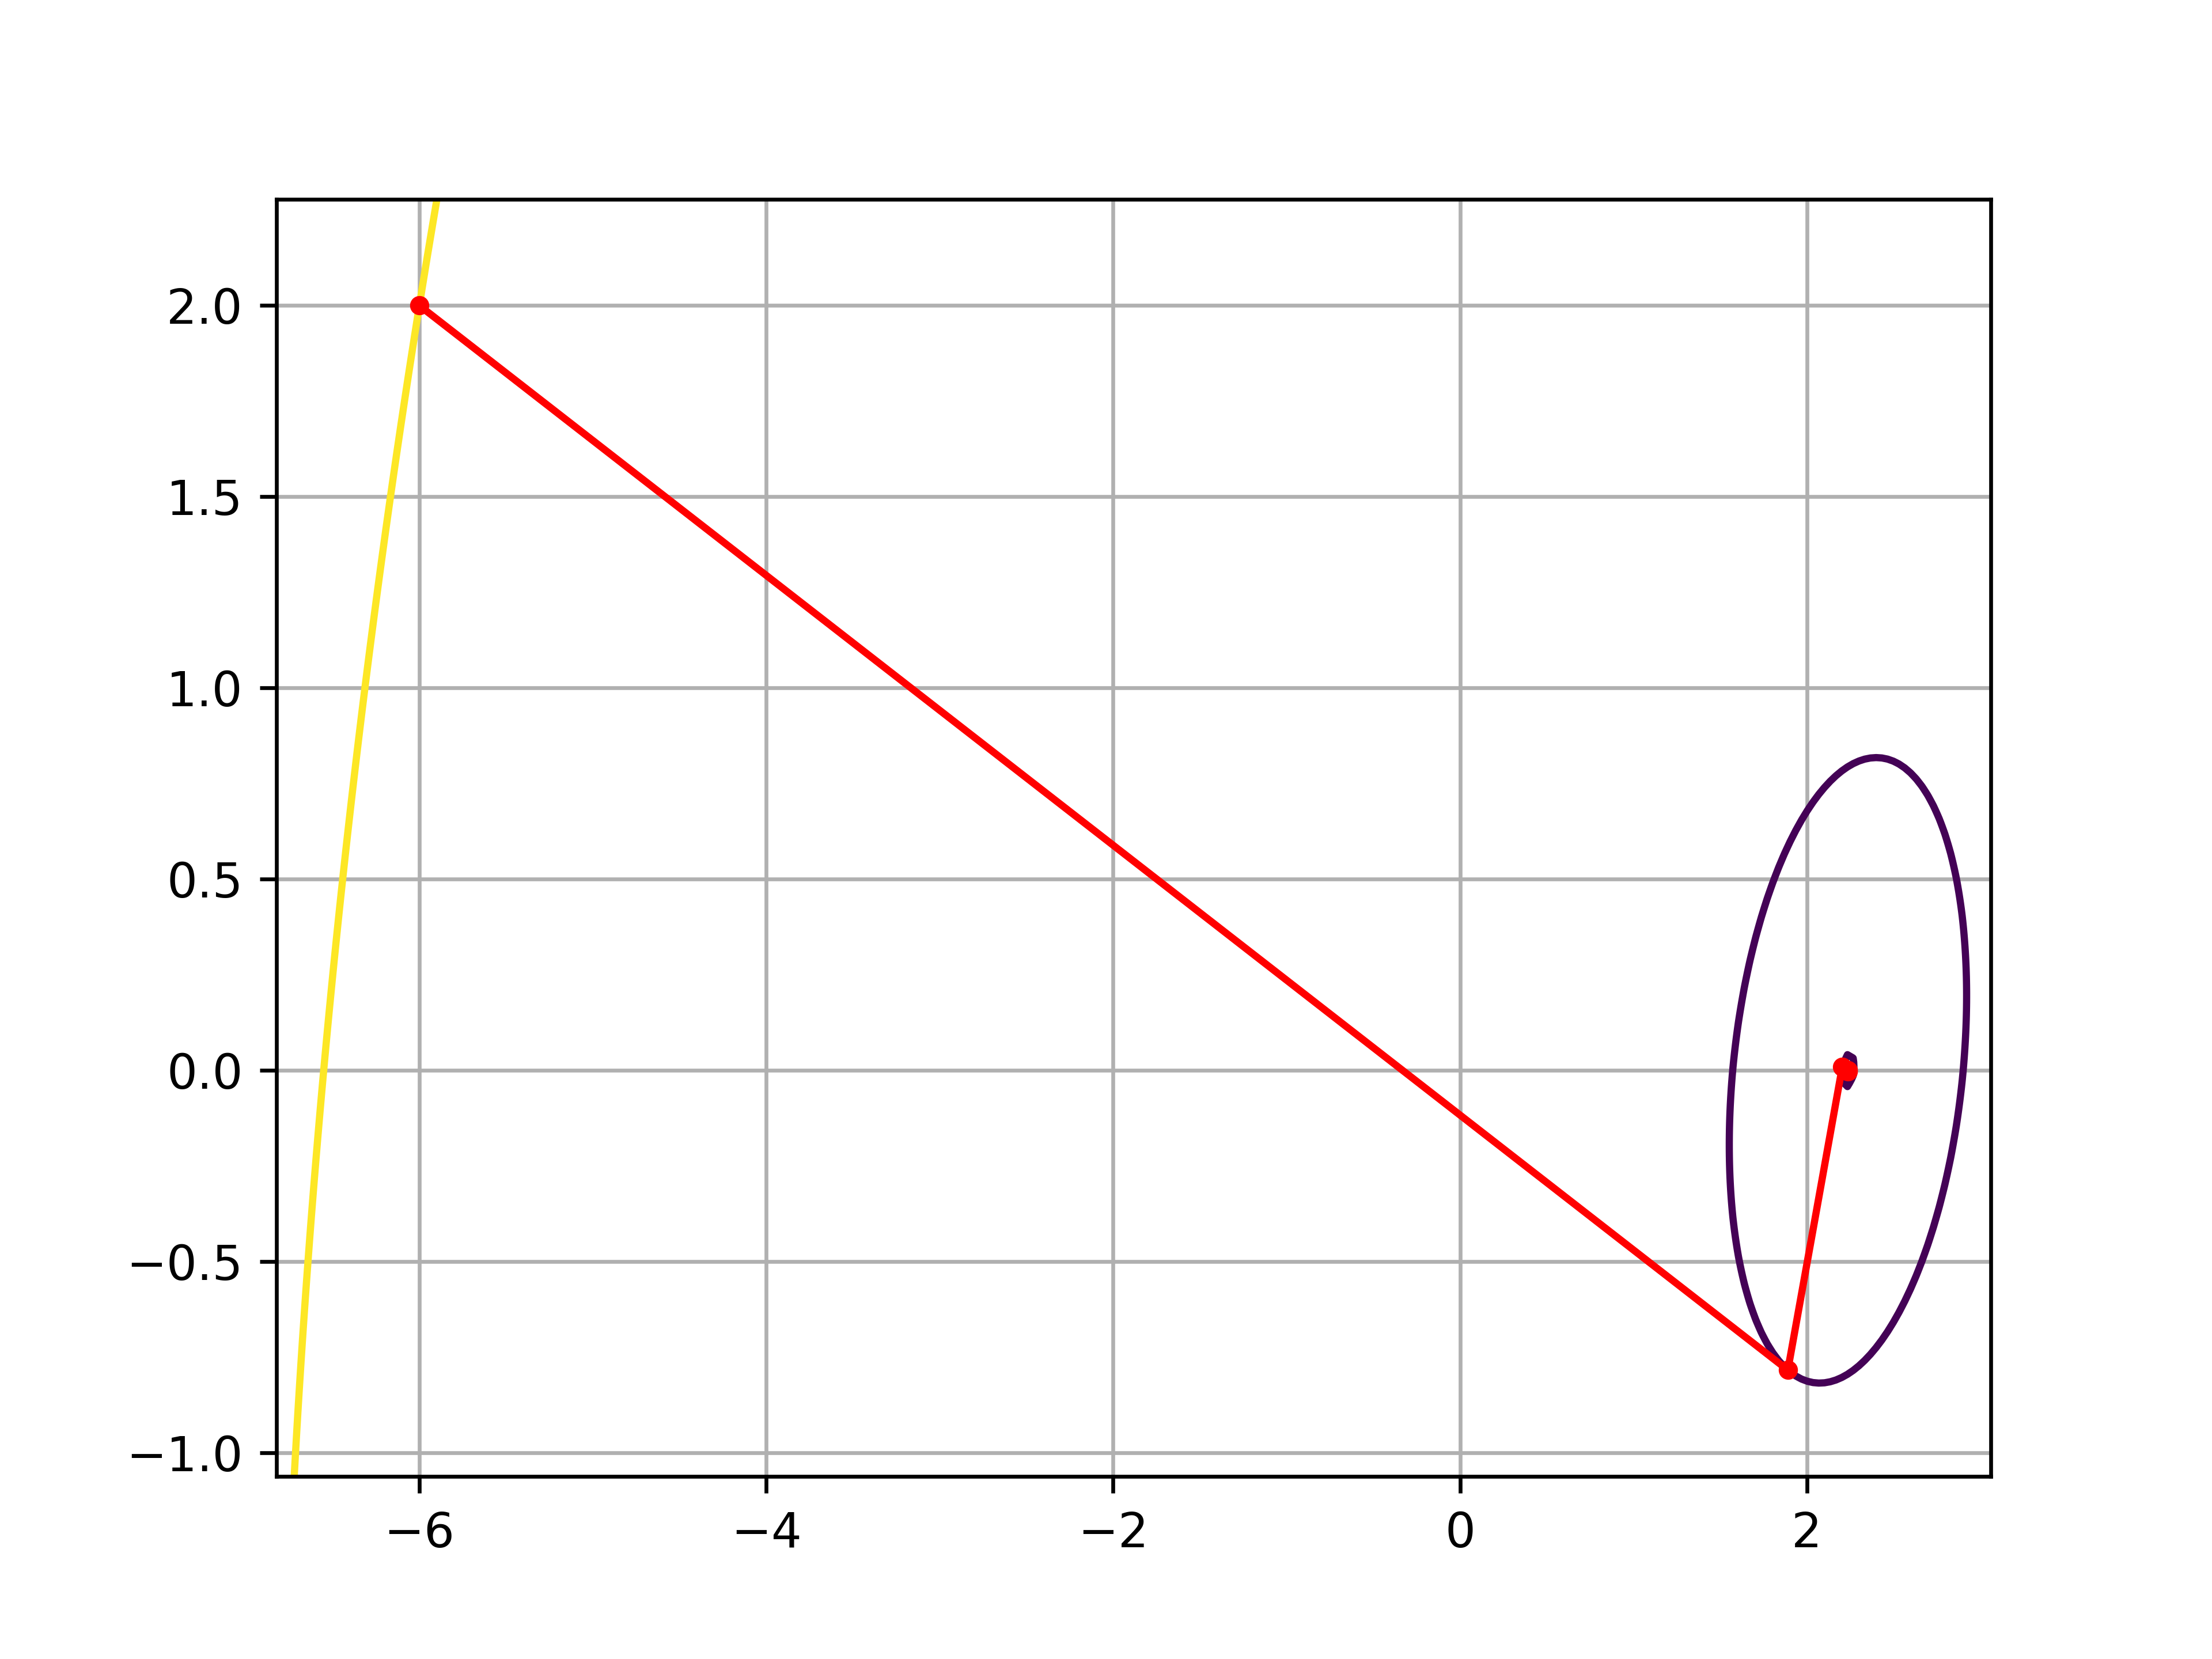
\includegraphics[width=0.85\textwidth]{Метод наискорейшего спуска, eps 0.01, start = (-6.00, 2.00), Квадратичная функция}%
	        \caption{Поиск минимума квадратичной функции при $\varepsilon = 0.01$, начальной точке (-6.0, 2.0) методом наискорейшего спуска}
	        \vspace*{-1.2cm}
            \end{figure}
            
            \begin{figure}[H]
	        \centering
	        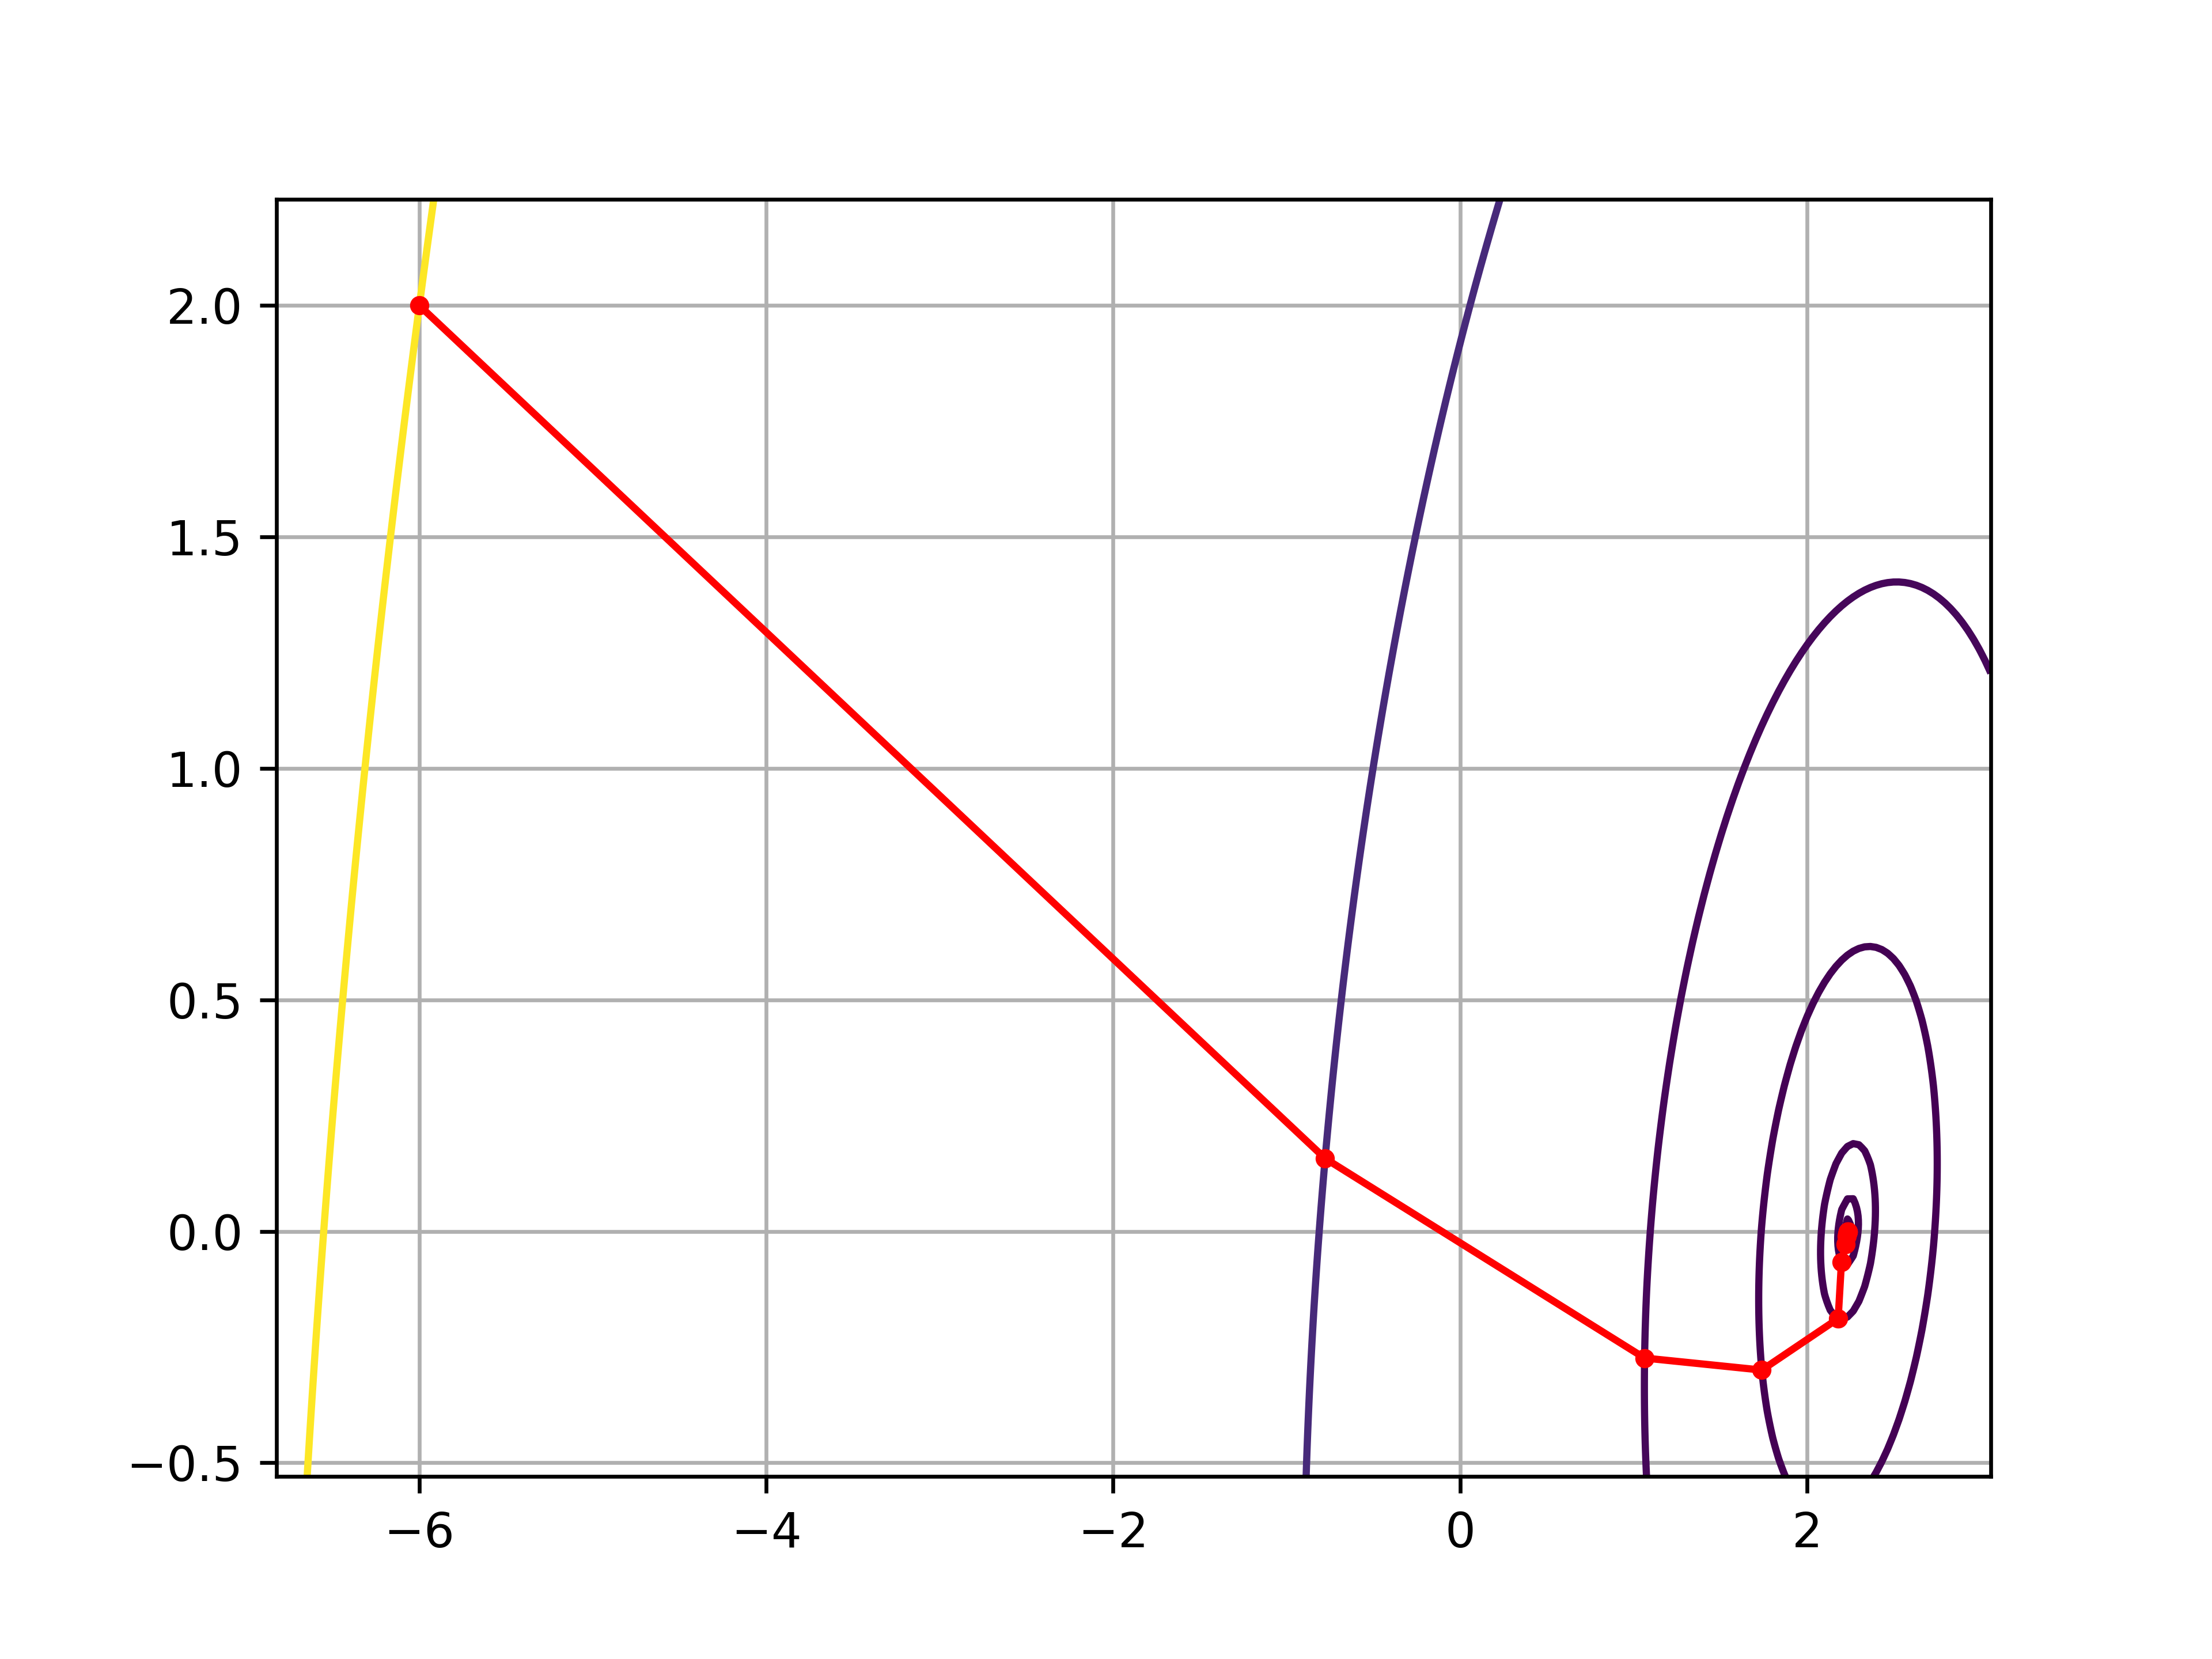
\includegraphics[width=0.85\textwidth]{Метод градиентного спуска с дробным шагом, eps 0.01, start = (-6.00, 2.00), Квадратичная функция}%
	        \caption{Поиск минимума квадратичной функции при $\varepsilon = 0.01$, начальной точке (-6.0, 2.0) методом градиентного спуска с дроблением шага}
	        \vspace*{-1.2cm}
            \end{figure}
            
            \begin{figure}[H]
	        \centering
	        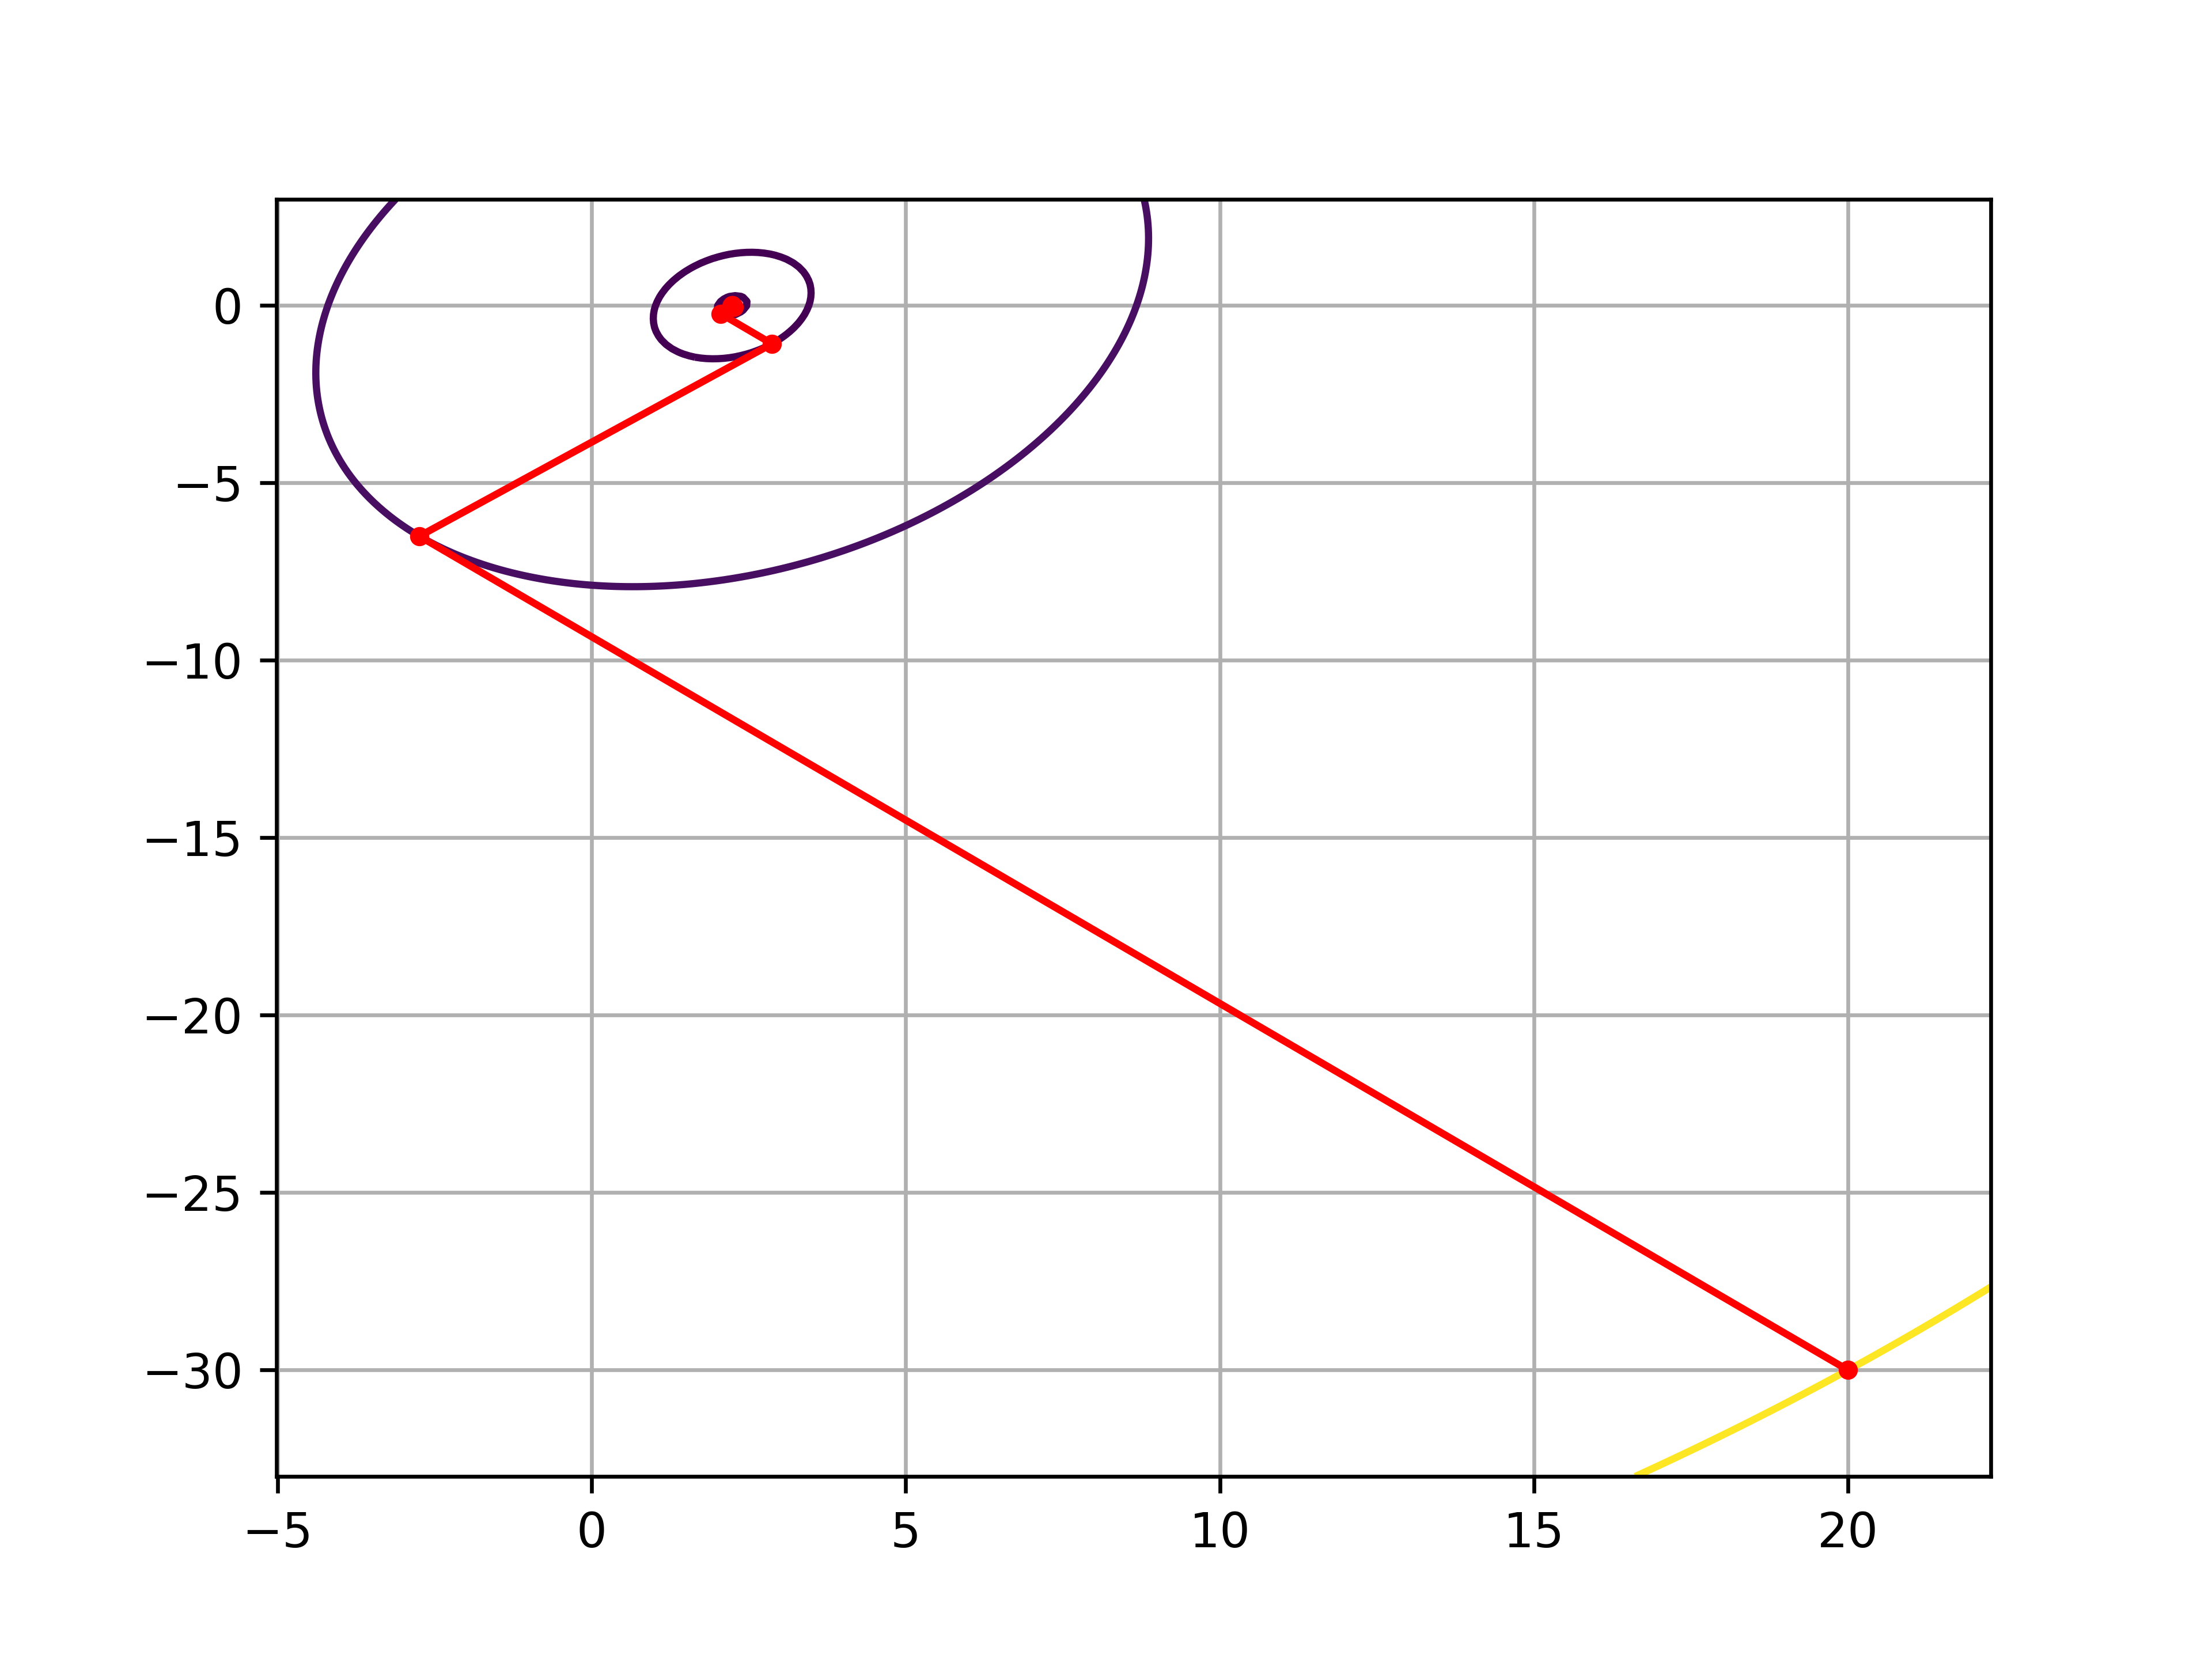
\includegraphics[width=0.85\textwidth]{Метод наискорейшего спуска, eps 0.01, start = (20.00, -30.00), Квадратичная функция}%
	        \caption{Поиск минимума квадратичной функции при $\varepsilon = 0.01$, начальной точке (20.0, -30.0) методом наискорейшего спуска}
	        \vspace*{-1.2cm}
            \end{figure}
            
            \begin{figure}[H]
	        \centering
	        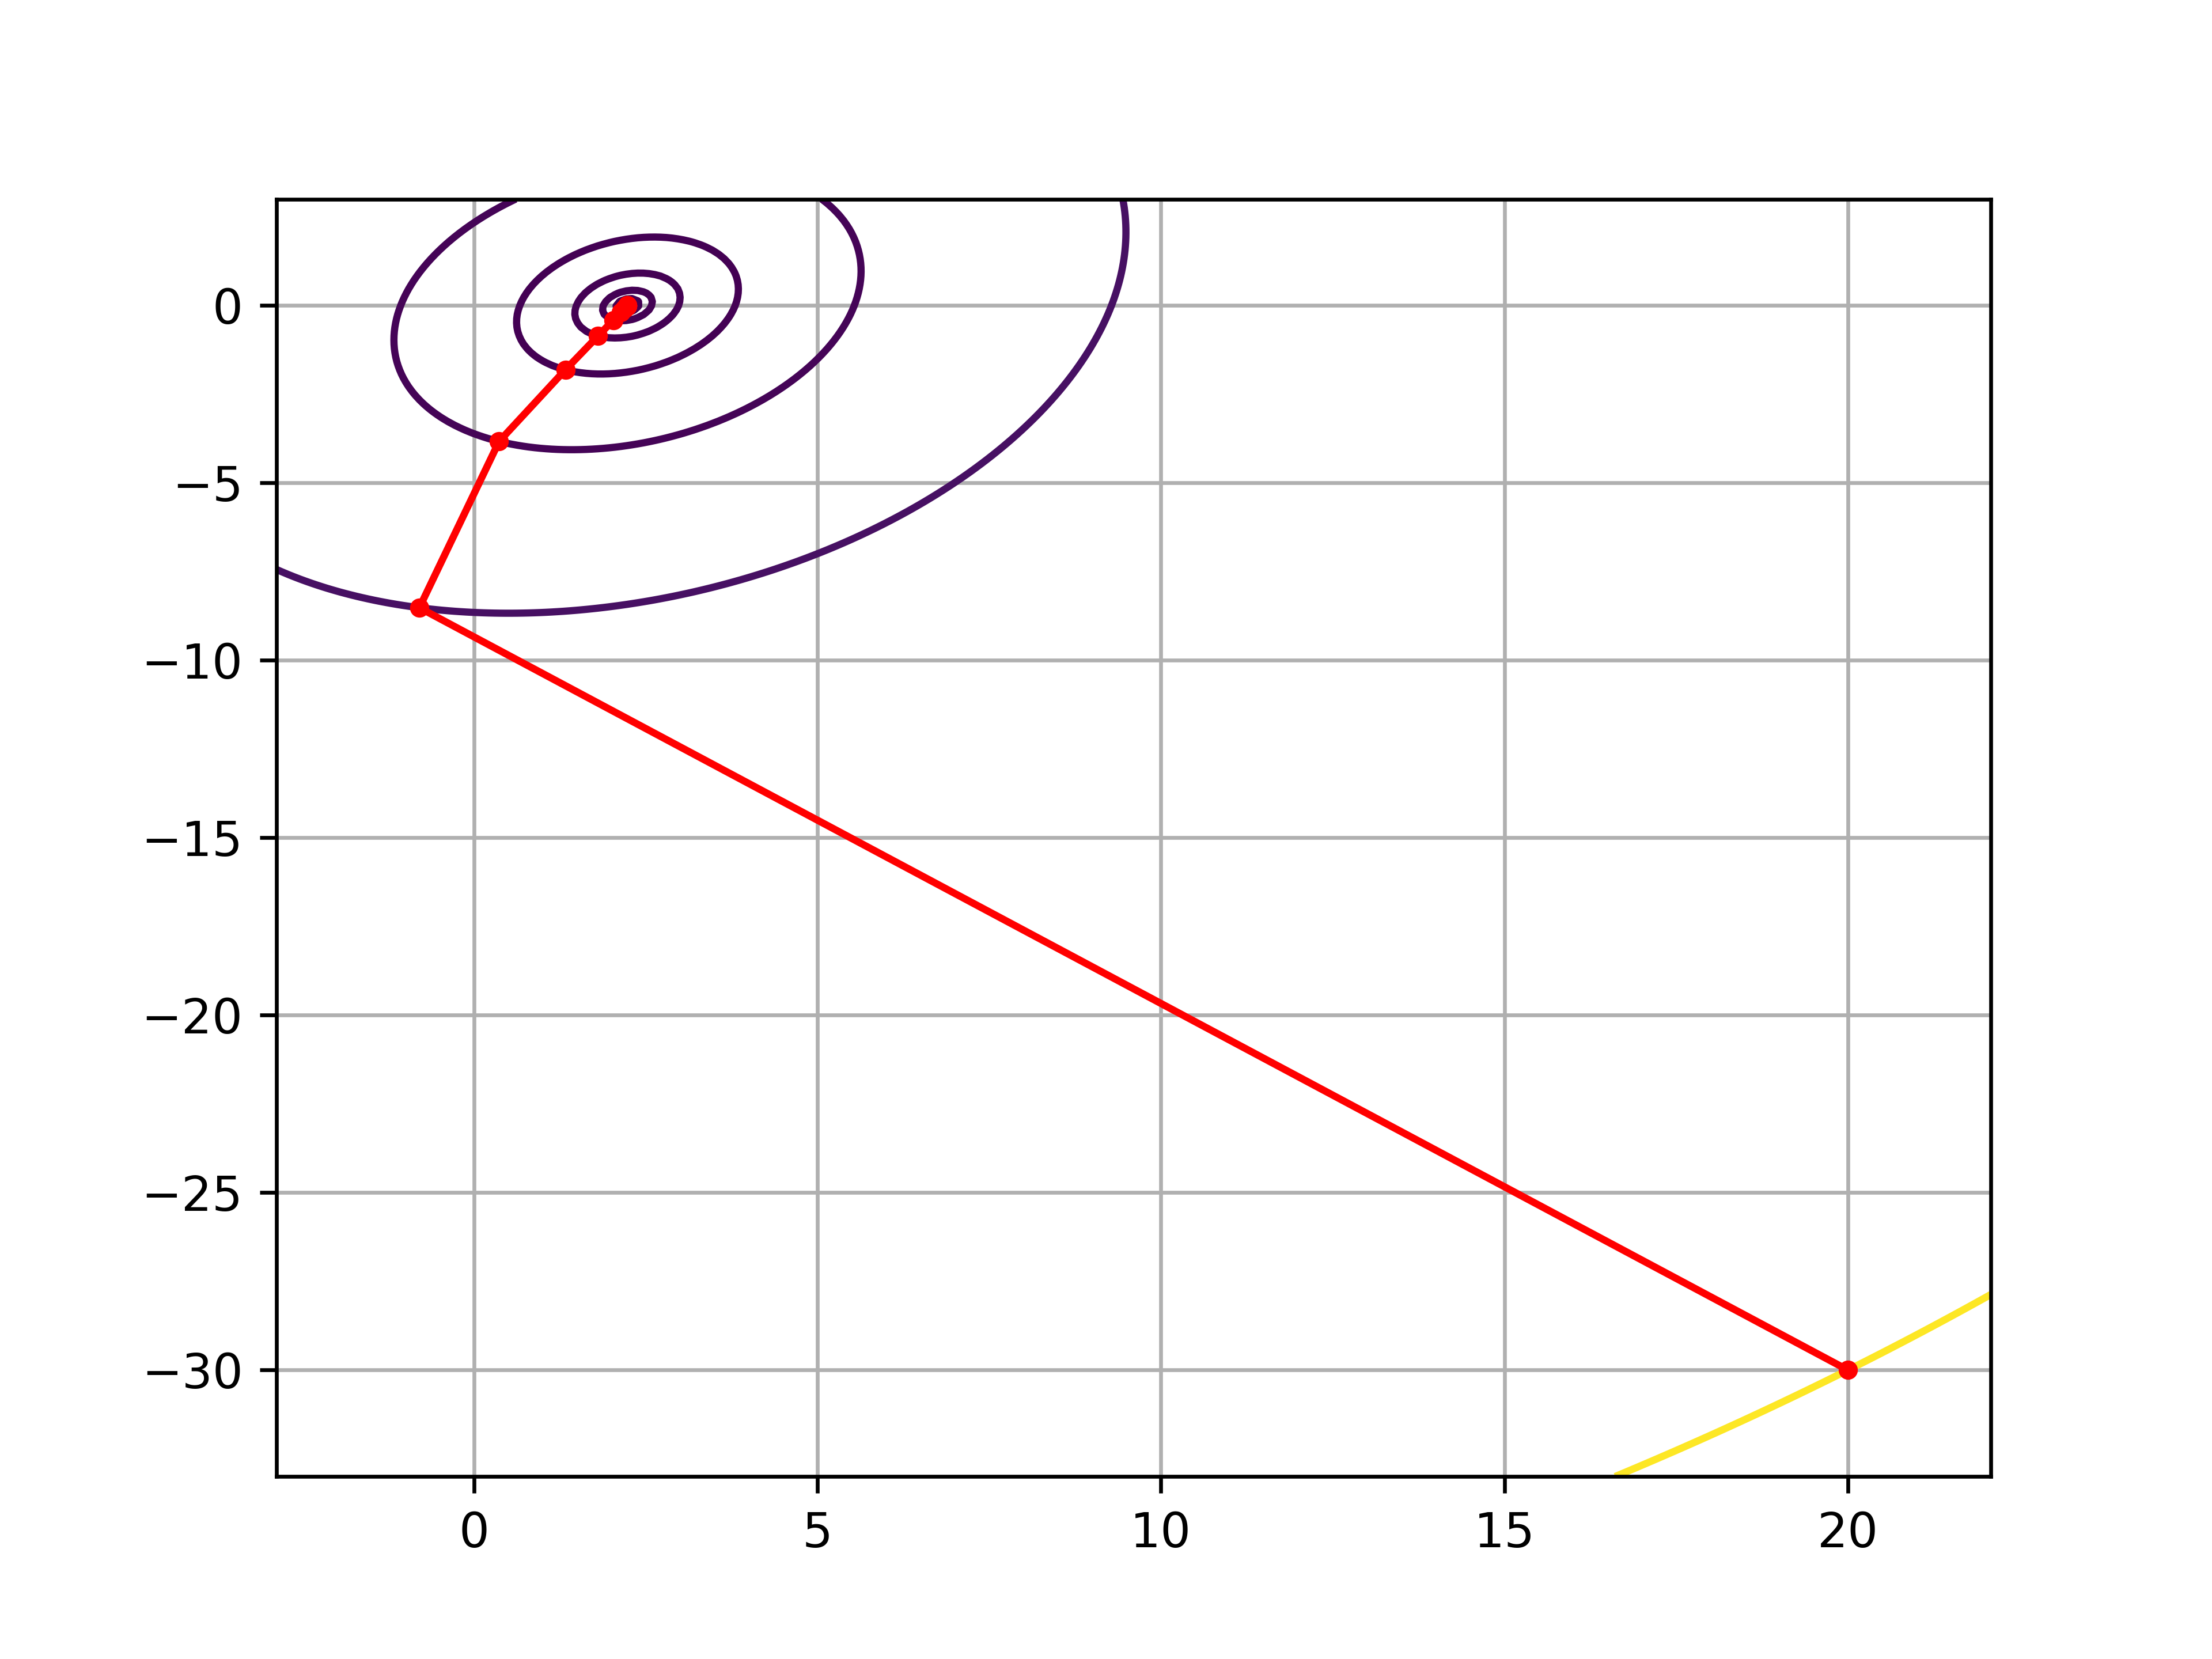
\includegraphics[width=0.85\textwidth]{Метод градиентного спуска с дробным шагом, eps 0.01, start = (20.00, -30.00), Квадратичная функция}%
	        \caption{Поиск минимума квадратичной функции при $\varepsilon = 0.01$, начальной точке (20.0, -30.0) методом градиентного спуска с дроблением шага}
	        \vspace*{-1.2cm}
            \end{figure}
            
            \begin{figure}[H]
	        \centering
	        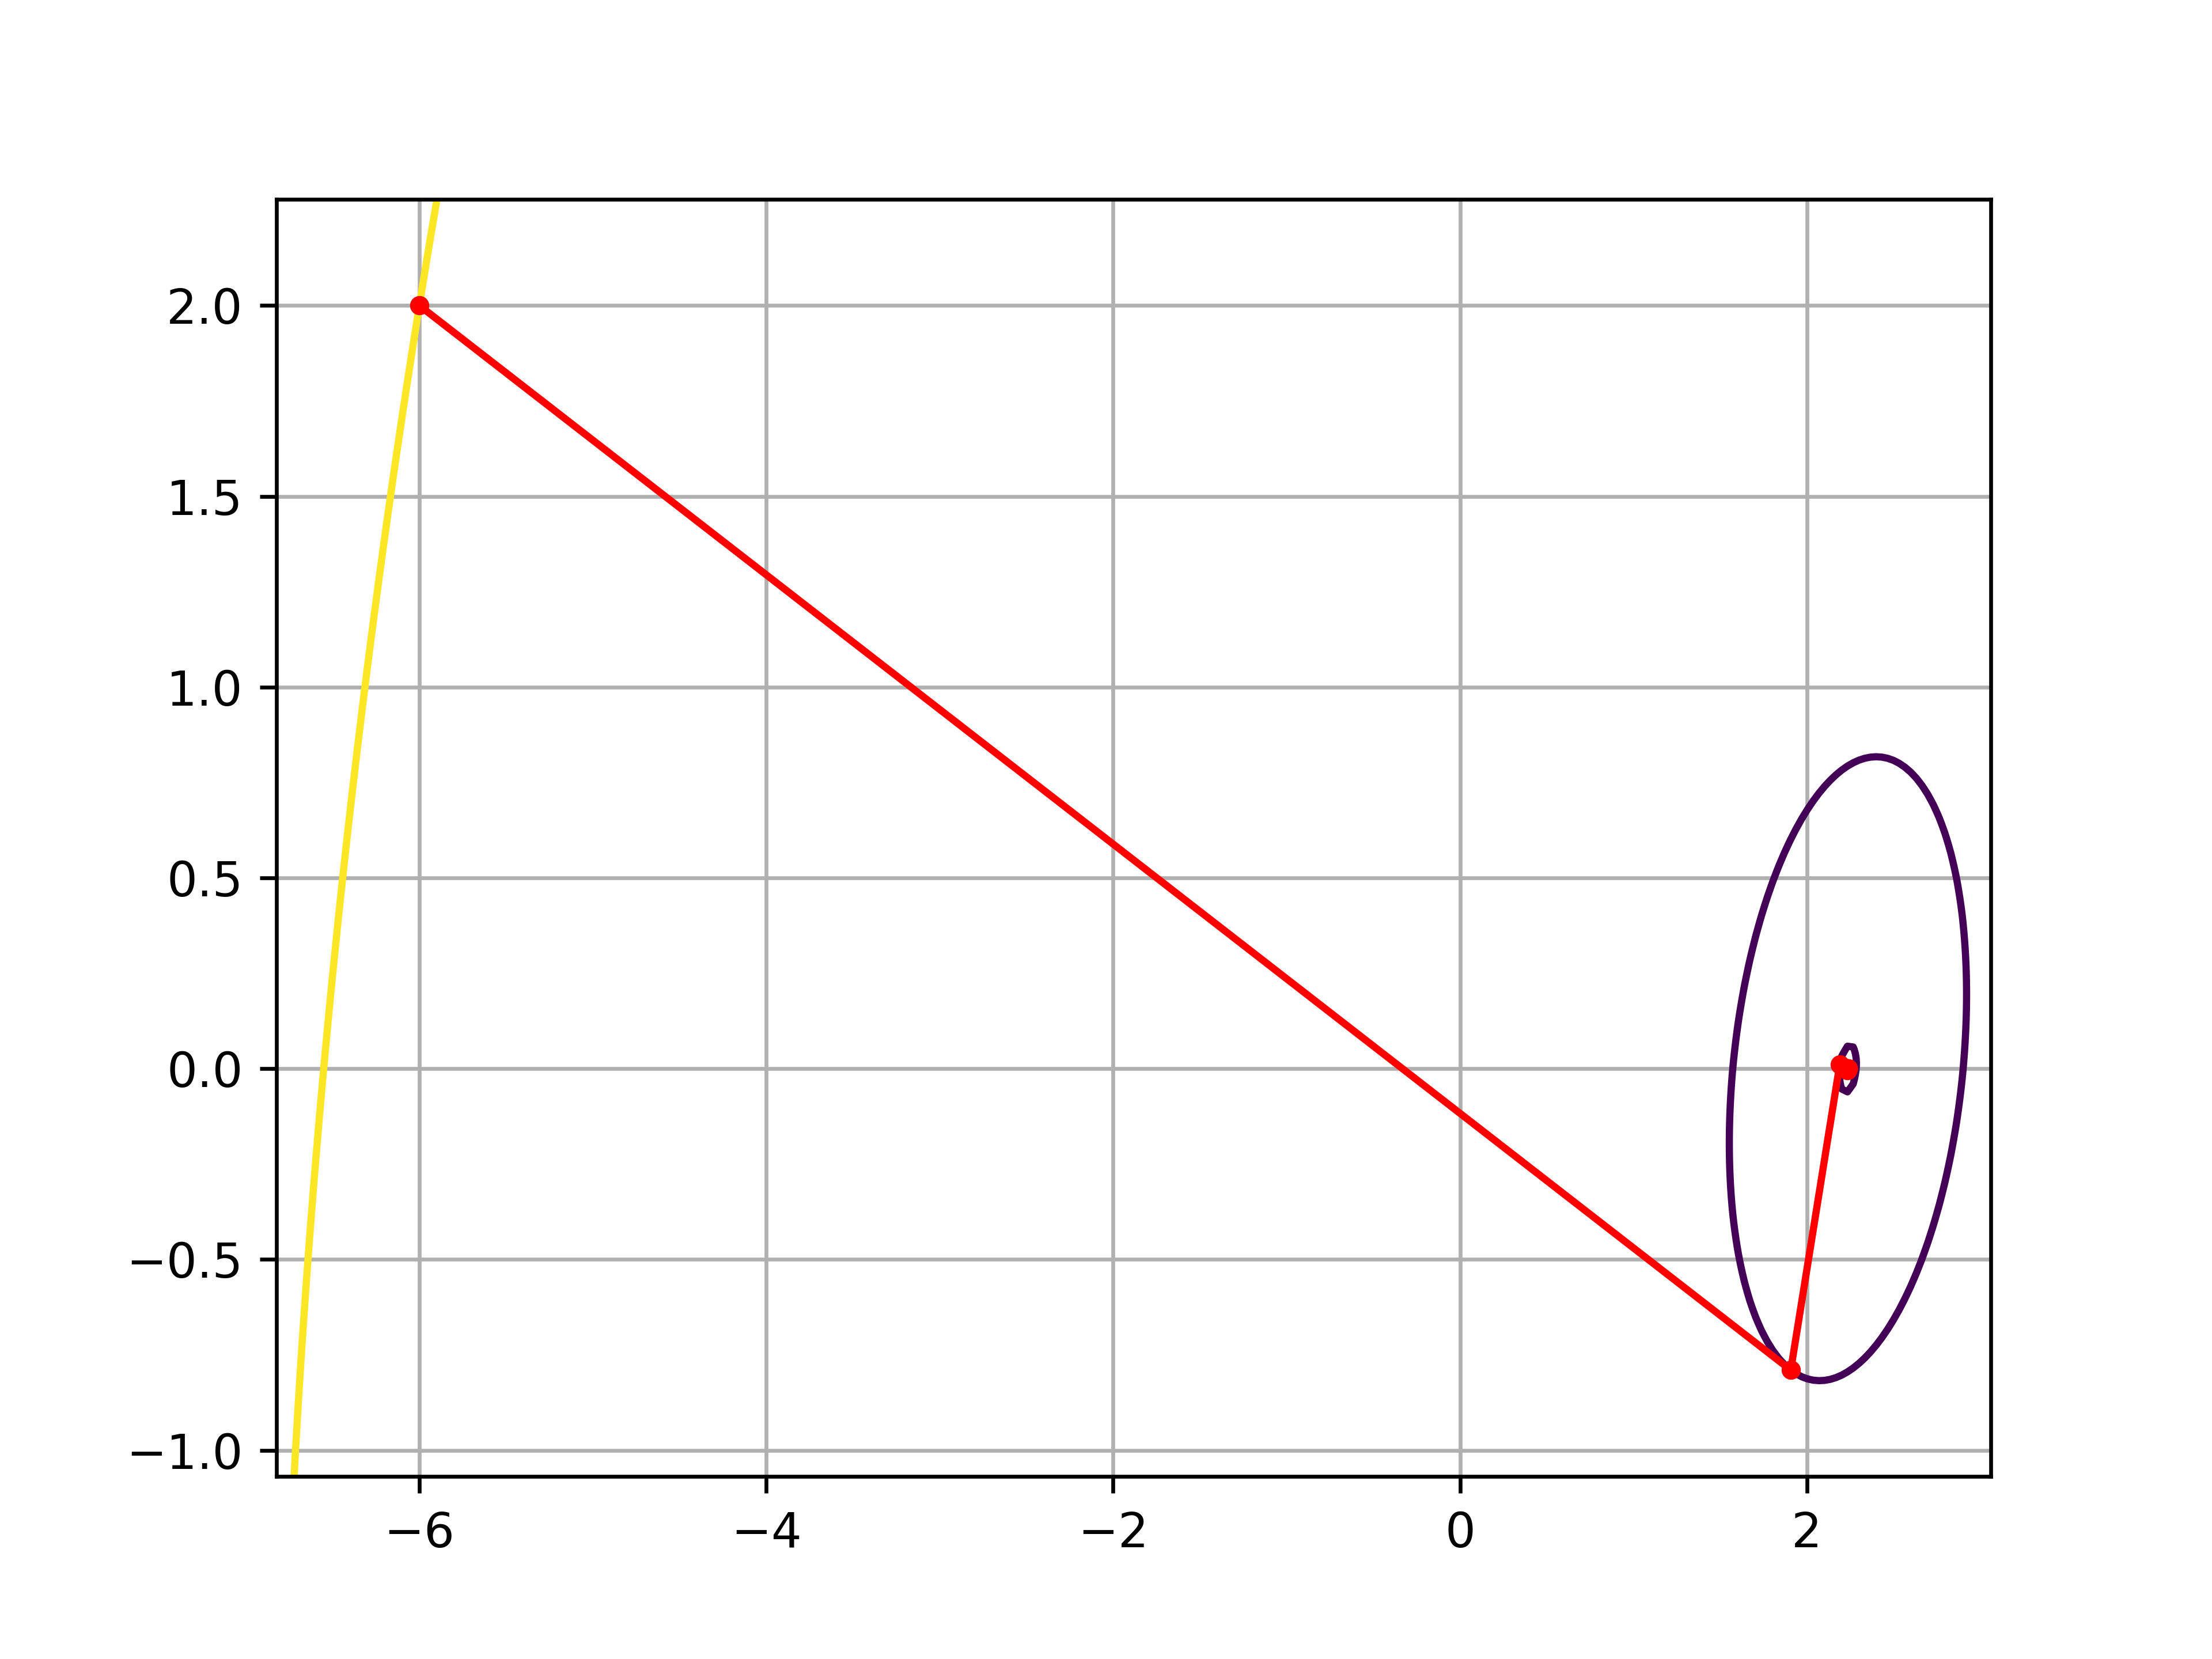
\includegraphics[width=0.85\textwidth]{Метод наискорейшего спуска, eps 1e-06, start = (-6.000000, 2.000000), Квадратичная функция}%
	        \caption{Поиск минимума квадратичной функции при $\varepsilon = 1e-06$, начальной точке (-6.0, 2.0) методом наискорейшего спуска}
	        \vspace*{-1.2cm}
            \end{figure}
            
            \begin{figure}[H]
	        \centering
	        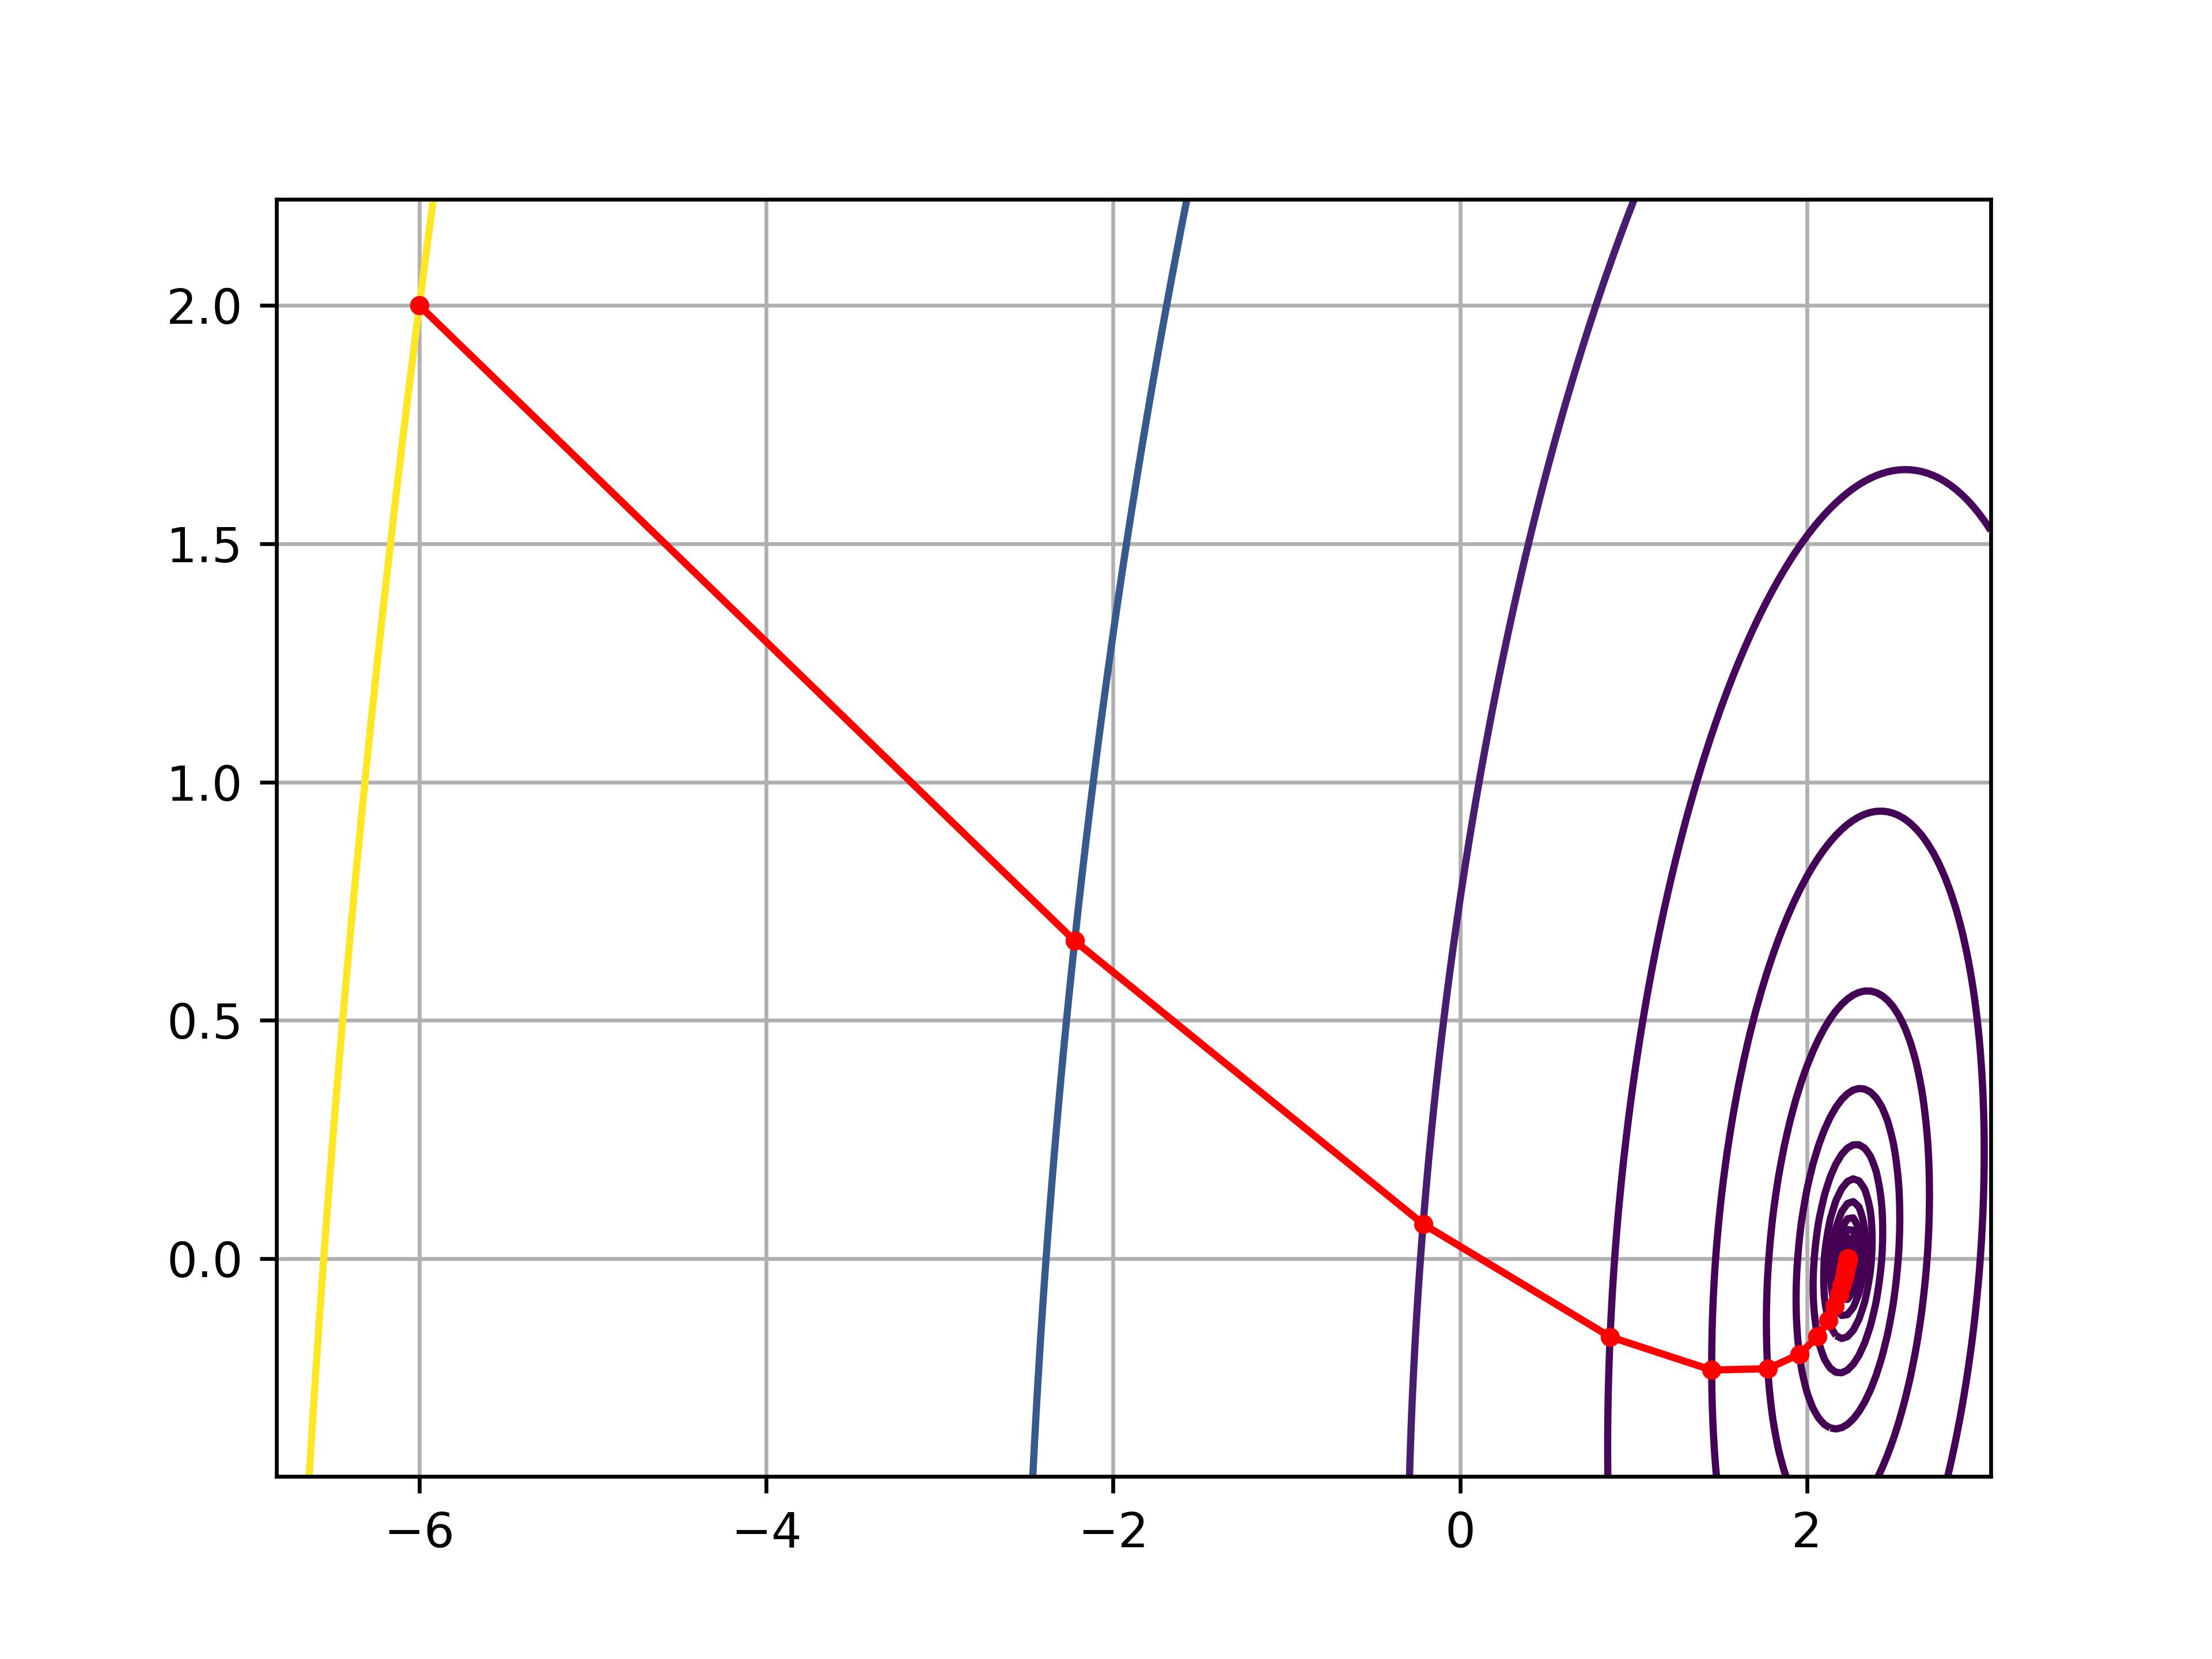
\includegraphics[width=0.85\textwidth]{Метод градиентного спуска с дробным шагом, eps 1e-06, start = (-6.000000, 2.000000), Квадратичная функция}%
	        \caption{Поиск минимума квадратичной функции при $\varepsilon = 1e-06$, начальной точке (-6.0, 2.0) методом градиентного спуска с дроблением шага}
	        \vspace*{-1.2cm}
            \end{figure}
            
            \begin{figure}[H]
	        \centering
	        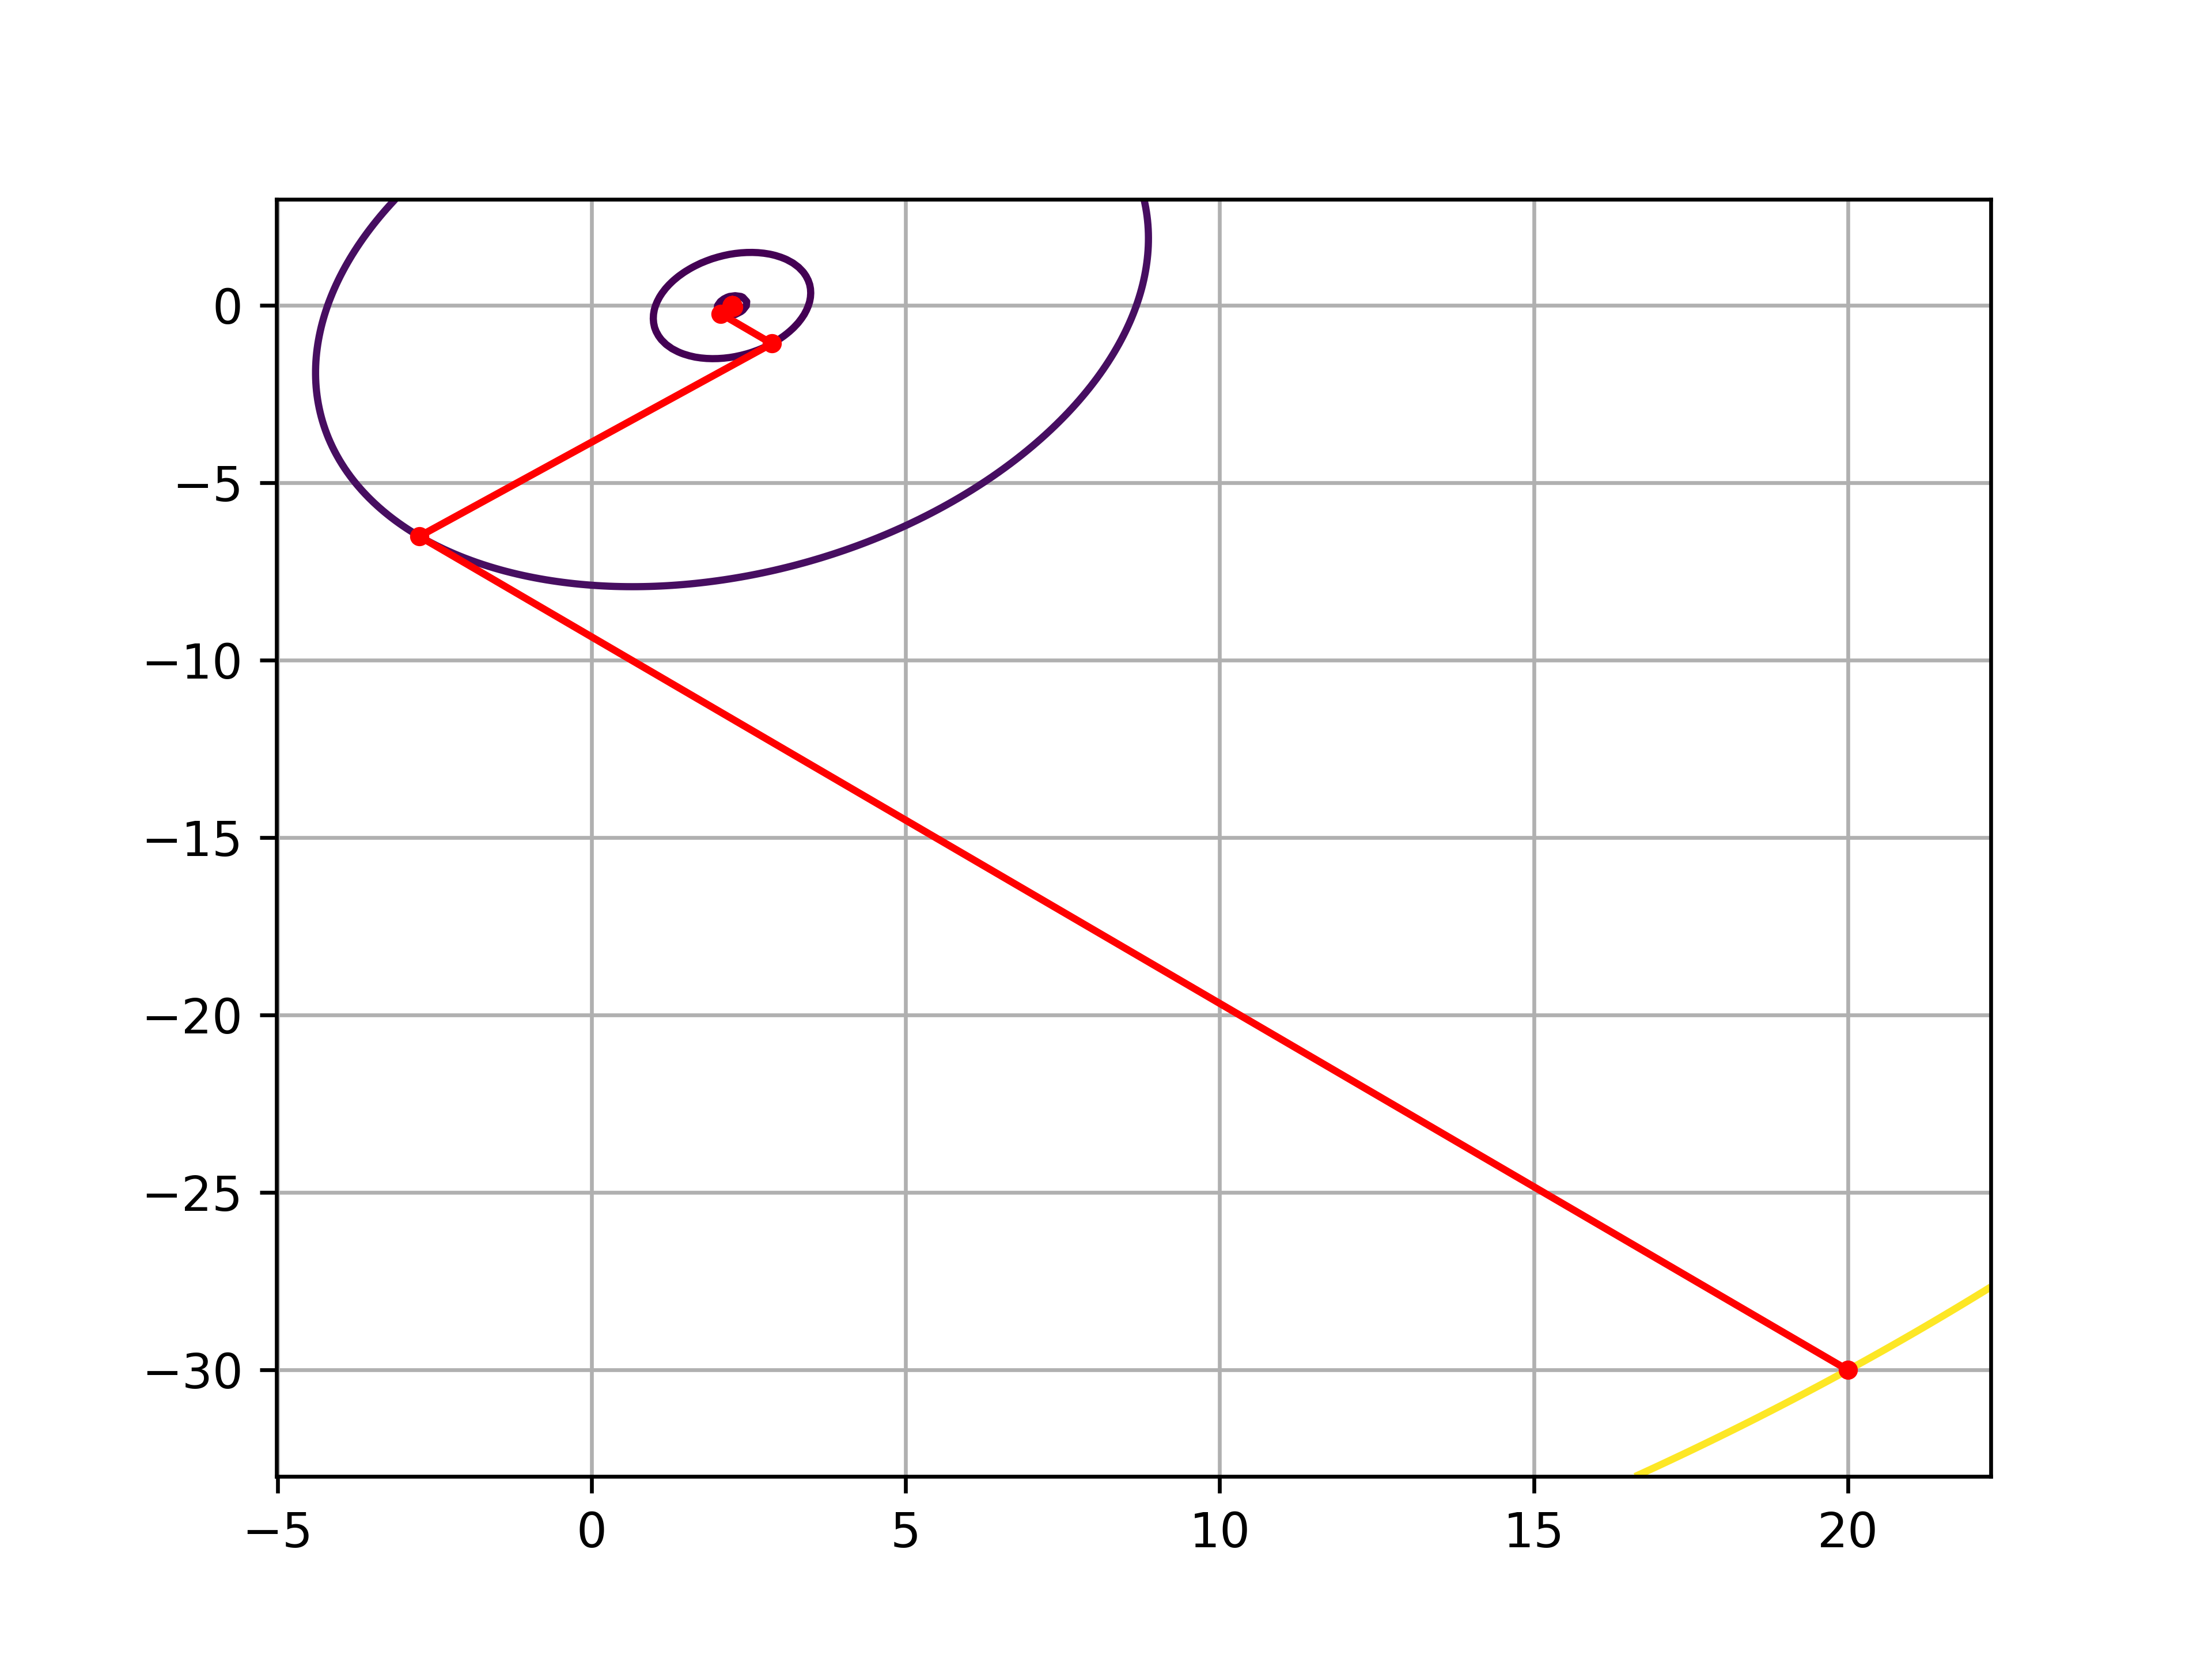
\includegraphics[width=0.85\textwidth]{Метод наискорейшего спуска, eps 1e-06, start = (20.000000, -30.000000), Квадратичная функция}%
	        \caption{Поиск минимума квадратичной функции при $\varepsilon = 1e-06$, начальной точке (20.0, -30.0) методом наискорейшего спуска}
	        \vspace*{-1.2cm}
            \end{figure}
            
            \begin{figure}[H]
	        \centering
	        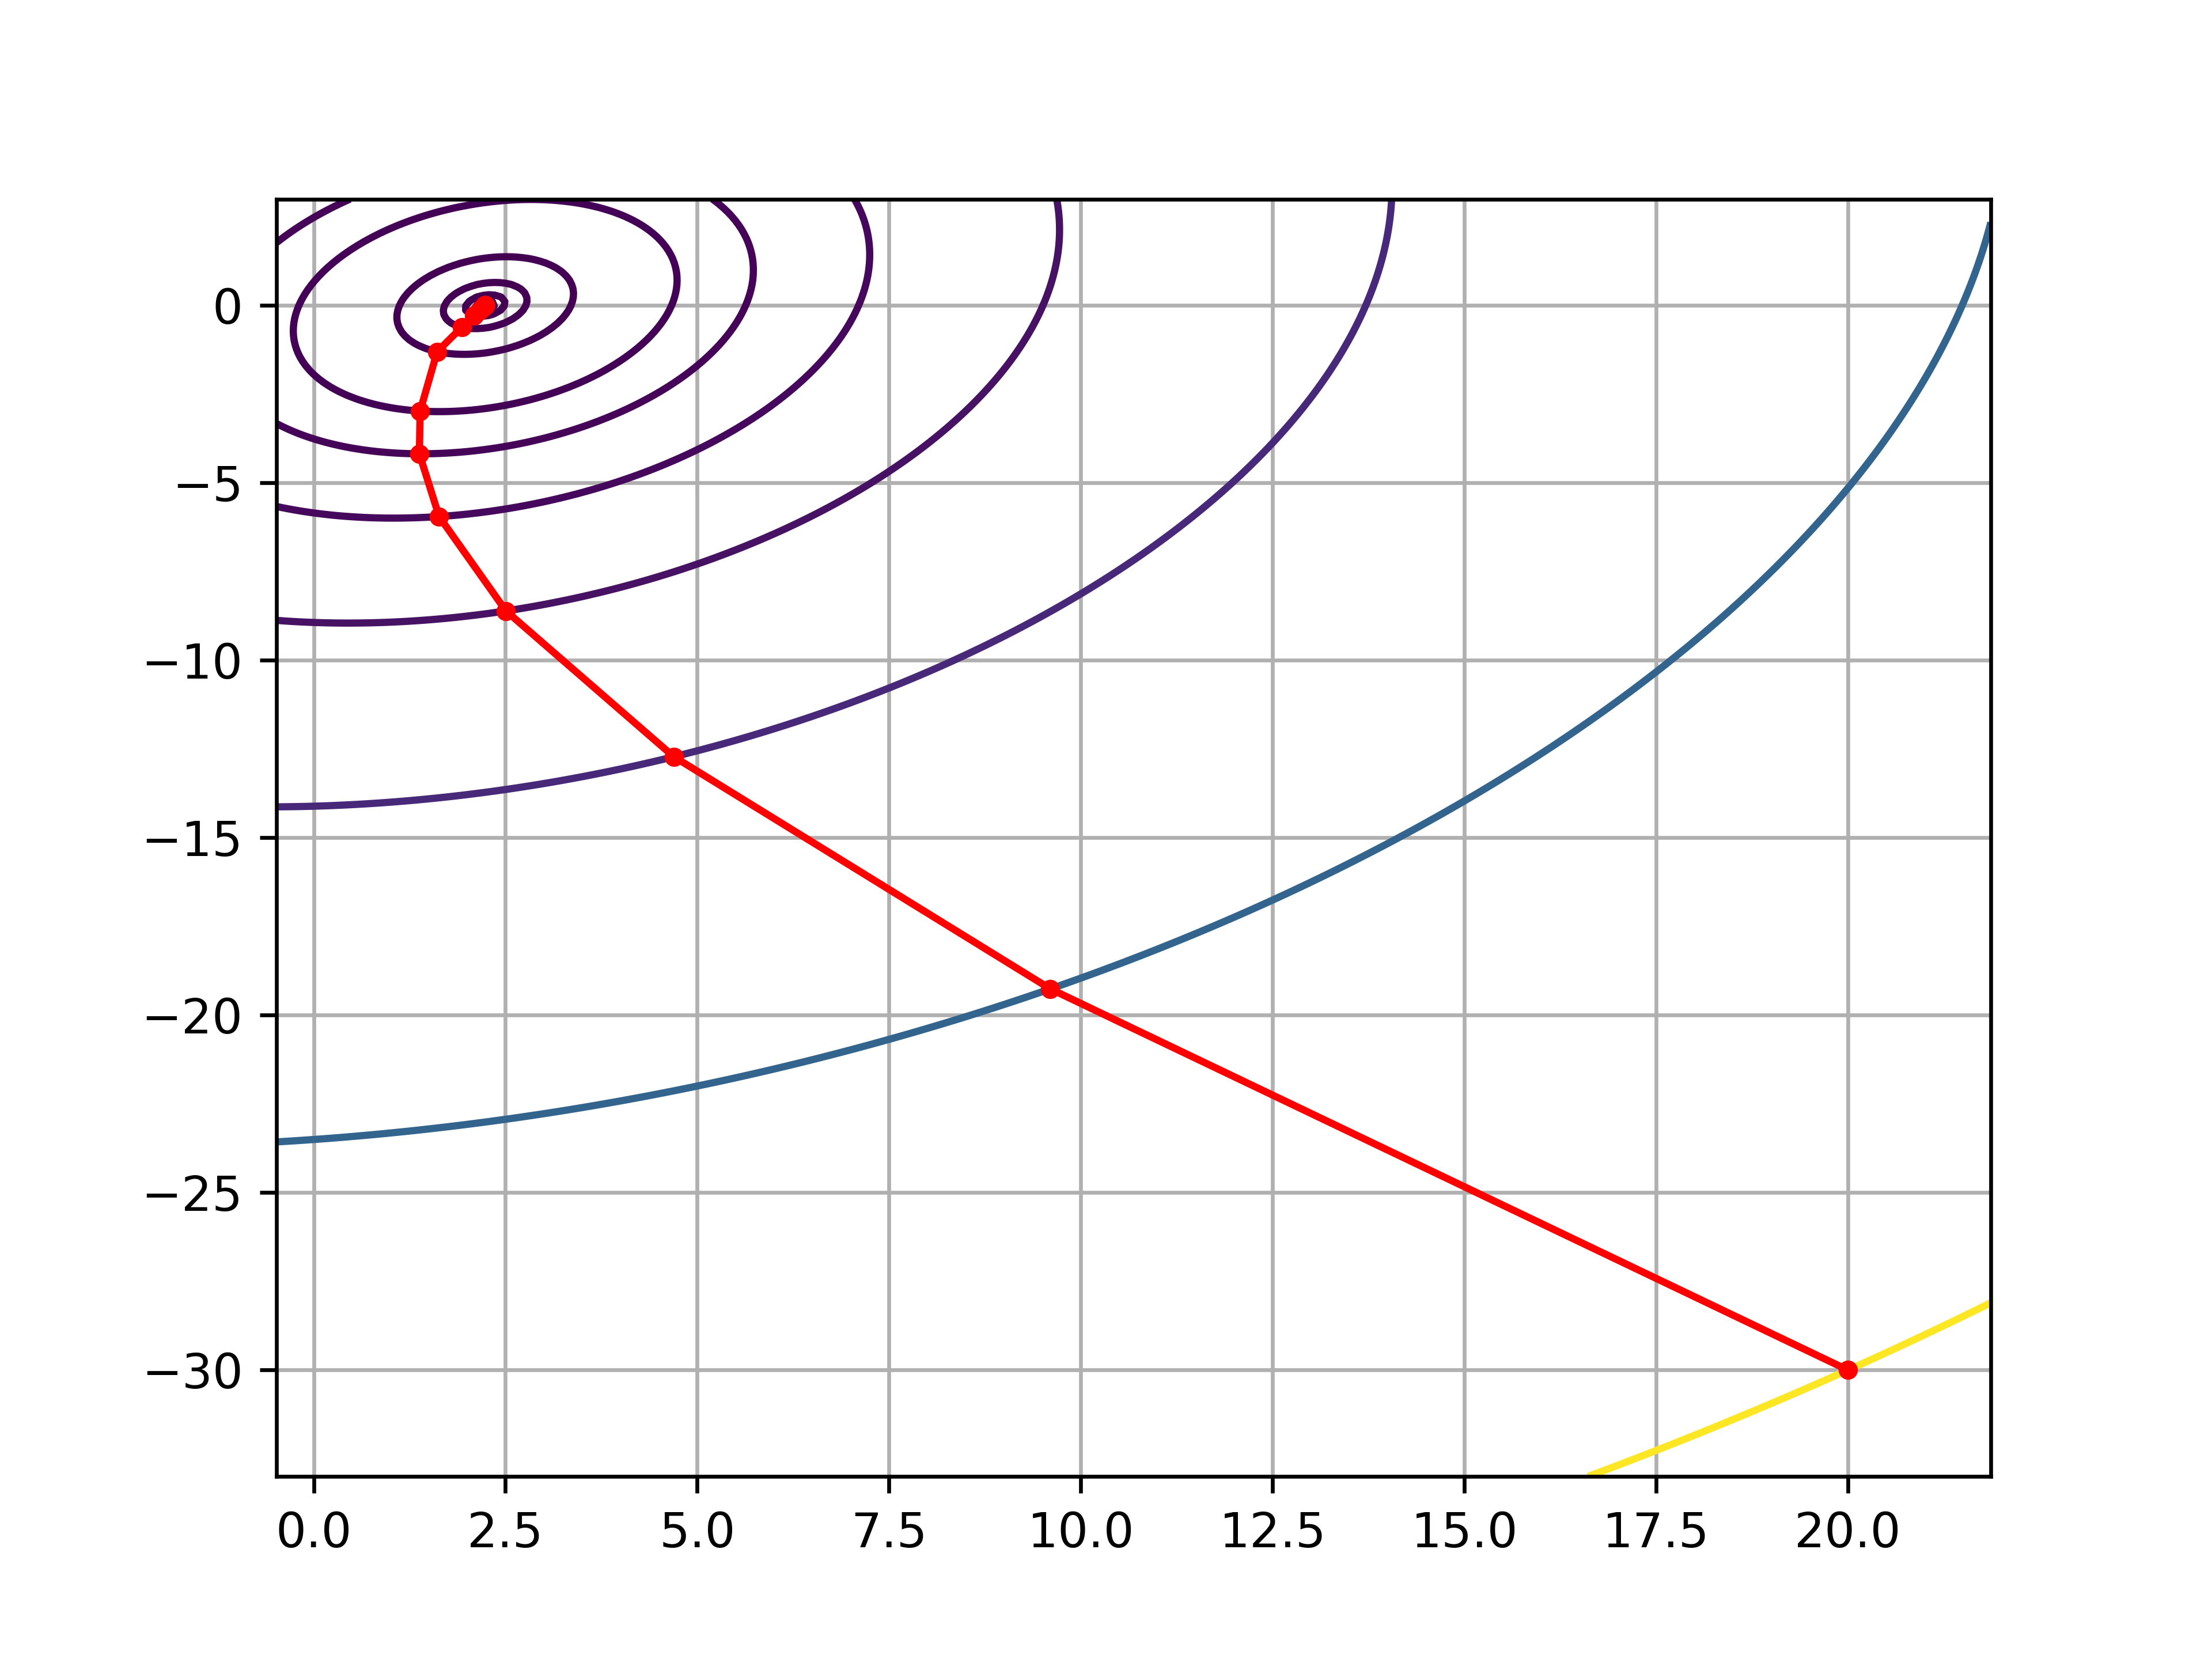
\includegraphics[width=0.85\textwidth]{Метод градиентного спуска с дробным шагом, eps 1e-06, start = (20.000000, -30.000000), Квадратичная функция}%
	        \caption{Поиск минимума квадратичной функции при $\varepsilon = 1e-06$, начальной точке (20.0, -30.0) методом градиентного спуска с дроблением шага}
	        \vspace*{-1.2cm}
            \end{figure}
            \subsubsection{Функция Розенброка с $\alpha$ = 1}

\begin{table}[H]
        \centering
        \vspace*{-1.5em}
        \caption{Результаты работы алгоритмов\\для функции Розенброка с $\alpha$ = 1}
        \footnotesize
        \begin{tabular}{|c|c|c|c|}
        \hline
        & &\makecell{Метод наискорейшего\\спуска} &\makecell{Метод градиентного спуска\\с дроблением шага} \\
        \hline
	\multirow{10}{*}{\rotatebox[origin=c]{90}{$\varepsilon = 0.01$}}&\textbf{Начальная точка} &\multicolumn{2}{c|}{\textbf{(-6.00, 2.00)}}\\
	\cline{2-4}
	&Точка минимума &(1.01, 1.02) &(1.01, 1.02) \\ 
	\cline{2-4}
	&Минимум &0.00 &0.00 \\ 
	\cline{2-4}
	&Кол-во итераций &107 &33 \\ 
	\cline{2-4}
	&\makecell{Кол-во вызовов\\целевой функции} &1960 &268 \\ 
	\cline{2-4}
	&\makecell{Кол-во вычислений\\градиента} &107 &33 \\ 
	\cline{2-4}
\cline{2-4}&\textbf{Начальная точка} &\multicolumn{2}{c|}{\textbf{(20.00, -30.00)}}\\
	\cline{2-4}
	&Точка минимума &(1.01, 1.02) &(1.00, 0.99) \\ 
	\cline{2-4}
	&Минимум &0.00 &0.00 \\ 
	\cline{2-4}
	&Кол-во итераций &98 &35 \\ 
	\cline{2-4}
	&\makecell{Кол-во вызовов\\целевой функции} &1765 &320 \\ 
	\cline{2-4}
	&\makecell{Кол-во вычислений\\градиента} &98 &35 \\ 
	\cline{2-4}
	\hline
	\multirow{10}{*}{\rotatebox[origin=c]{90}{$\varepsilon = 1e-06$}}&\textbf{Начальная точка} &\multicolumn{2}{c|}{\textbf{(-6.000000, 2.000000)}}\\
	\cline{2-4}
	&Точка минимума &(1.000001, 1.000002) &(1.000000, 1.000001) \\ 
	\cline{2-4}
	&Минимум &0.000000 &0.000000 \\ 
	\cline{2-4}
	&Кол-во итераций &172 &69 \\ 
	\cline{2-4}
	&\makecell{Кол-во вызовов\\целевой функции} &6304 &512 \\ 
	\cline{2-4}
	&\makecell{Кол-во вычислений\\градиента} &172 &69 \\ 
	\cline{2-4}
\cline{2-4}&\textbf{Начальная точка} &\multicolumn{2}{c|}{\textbf{(20.000000, -30.000000)}}\\
	\cline{2-4}
	&Точка минимума &(0.999999, 0.999998) &(1.000000, 0.999999) \\ 
	\cline{2-4}
	&Минимум &0.000000 &0.000000 \\ 
	\cline{2-4}
	&Кол-во итераций &102 &55 \\ 
	\cline{2-4}
	&\makecell{Кол-во вызовов\\целевой функции} &3718 &441 \\ 
	\cline{2-4}
	&\makecell{Кол-во вычислений\\градиента} &102 &55 \\ 
	\cline{2-4}
	\hline

\end{tabular}
\end{table}


            \begin{figure}[H]
	        \centering
	        \includegraphics[width=0.85\textwidth]{Метод наискорейшего спуска, eps 0.01, start = (-6.00, 2.00), Функция Розенброка с alpha = 1}%
	        \caption{Поиск минимума функции Розенброка с $\alpha$ = 1 при $\varepsilon = 0.01$, начальной точке (-6.0, 2.0) методом наискорейшего спуска}
	        \vspace*{-1.2cm}
            \end{figure}
            
            \begin{figure}[H]
	        \centering
	        \includegraphics[width=0.85\textwidth]{Метод градиентного спуска с дробным шагом, eps 0.01, start = (-6.00, 2.00), Функция Розенброка с alpha = 1}%
	        \caption{Поиск минимума функции Розенброка с $\alpha$ = 1 при $\varepsilon = 0.01$, начальной точке (-6.0, 2.0) методом градиентного спуска с дроблением шага}
	        \vspace*{-1.2cm}
            \end{figure}
            
            \begin{figure}[H]
	        \centering
	        \includegraphics[width=0.85\textwidth]{Метод наискорейшего спуска, eps 0.01, start = (20.00, -30.00), Функция Розенброка с alpha = 1}%
	        \caption{Поиск минимума функции Розенброка с $\alpha$ = 1 при $\varepsilon = 0.01$, начальной точке (20.0, -30.0) методом наискорейшего спуска}
	        \vspace*{-1.2cm}
            \end{figure}
            
            \begin{figure}[H]
	        \centering
	        \includegraphics[width=0.85\textwidth]{Метод градиентного спуска с дробным шагом, eps 0.01, start = (20.00, -30.00), Функция Розенброка с alpha = 1}%
	        \caption{Поиск минимума функции Розенброка с $\alpha$ = 1 при $\varepsilon = 0.01$, начальной точке (20.0, -30.0) методом градиентного спуска с дроблением шага}
	        \vspace*{-1.2cm}
            \end{figure}
            
            \begin{figure}[H]
	        \centering
	        \includegraphics[width=0.85\textwidth]{Метод наискорейшего спуска, eps 1e-06, start = (-6.000000, 2.000000), Функция Розенброка с alpha = 1}%
	        \caption{Поиск минимума функции Розенброка с $\alpha$ = 1 при $\varepsilon = 1e-06$, начальной точке (-6.0, 2.0) методом наискорейшего спуска}
	        \vspace*{-1.2cm}
            \end{figure}
            
            \begin{figure}[H]
	        \centering
	        \includegraphics[width=0.85\textwidth]{Метод градиентного спуска с дробным шагом, eps 1e-06, start = (-6.000000, 2.000000), Функция Розенброка с alpha = 1}%
	        \caption{Поиск минимума функции Розенброка с $\alpha$ = 1 при $\varepsilon = 1e-06$, начальной точке (-6.0, 2.0) методом градиентного спуска с дроблением шага}
	        \vspace*{-1.2cm}
            \end{figure}
            
            \begin{figure}[H]
	        \centering
	        \includegraphics[width=0.85\textwidth]{Метод наискорейшего спуска, eps 1e-06, start = (20.000000, -30.000000), Функция Розенброка с alpha = 1}%
	        \caption{Поиск минимума функции Розенброка с $\alpha$ = 1 при $\varepsilon = 1e-06$, начальной точке (20.0, -30.0) методом наискорейшего спуска}
	        \vspace*{-1.2cm}
            \end{figure}
            
            \begin{figure}[H]
	        \centering
	        \includegraphics[width=0.85\textwidth]{Метод градиентного спуска с дробным шагом, eps 1e-06, start = (20.000000, -30.000000), Функция Розенброка с alpha = 1}%
	        \caption{Поиск минимума функции Розенброка с $\alpha$ = 1 при $\varepsilon = 1e-06$, начальной точке (20.0, -30.0) методом градиентного спуска с дроблением шага}
	        \vspace*{-1.2cm}
            \end{figure}
            \subsubsection{Функция Розенброка с $\alpha$ = 10}

\begin{table}[H]
        \centering
        \vspace*{-1.5em}
        \caption{Результаты работы алгоритмов\\для функции Розенброка с $\alpha$ = 10}
        \footnotesize
        \begin{tabular}{|c|c|c|c|}
        \hline
        & &\makecell{Метод наискорейшего\\спуска} &\makecell{Метод градиентного спуска\\с дроблением шага} \\
        \hline
	\multirow{10}{*}{\rotatebox[origin=c]{90}{$\varepsilon = 0.01$}}&\textbf{Начальная точка} &\multicolumn{2}{c|}{\textbf{(-6.00, 2.00)}}\\
	\cline{2-4}
	&Точка минимума &(1.01, 1.02) &(1.01, 1.02) \\ 
	\cline{2-4}
	&Минимум &0.00 &0.00 \\ 
	\cline{2-4}
	&Кол-во итераций &191 &263 \\ 
	\cline{2-4}
	&\makecell{Кол-во вызовов\\целевой функции} &4091 &3142 \\ 
	\cline{2-4}
	&\makecell{Кол-во вычислений\\градиента} &191 &263 \\ 
	\cline{2-4}
\cline{2-4}&\textbf{Начальная точка} &\multicolumn{2}{c|}{\textbf{(20.00, -30.00)}}\\
	\cline{2-4}
	&Точка минимума &(1.01, 1.02) &(0.99, 0.98) \\ 
	\cline{2-4}
	&Минимум &0.00 &0.00 \\ 
	\cline{2-4}
	&Кол-во итераций &62 &79 \\ 
	\cline{2-4}
	&\makecell{Кол-во вызовов\\целевой функции} &1242 &908 \\ 
	\cline{2-4}
	&\makecell{Кол-во вычислений\\градиента} &62 &79 \\ 
	\cline{2-4}
	\hline
	\multirow{10}{*}{\rotatebox[origin=c]{90}{$\varepsilon = 1e-06$}}&\textbf{Начальная точка} &\multicolumn{2}{c|}{\textbf{(-6.000000, 2.000000)}}\\
	\cline{2-4}
	&Точка минимума &(1.000001, 1.000002) &(1.000001, 1.000002) \\ 
	\cline{2-4}
	&Минимум &0.000000 &0.000000 \\ 
	\cline{2-4}
	&Кол-во итераций &1522 &533 \\ 
	\cline{2-4}
	&\makecell{Кол-во вызовов\\целевой функции} &62699 &6197 \\ 
	\cline{2-4}
	&\makecell{Кол-во вычислений\\градиента} &1522 &533 \\ 
	\cline{2-4}
\cline{2-4}&\textbf{Начальная точка} &\multicolumn{2}{c|}{\textbf{(20.000000, -30.000000)}}\\
	\cline{2-4}
	&Точка минимума &(0.999999, 0.999998) &(0.999999, 0.999998) \\ 
	\cline{2-4}
	&Минимум &0.000000 &0.000000 \\ 
	\cline{2-4}
	&Кол-во итераций &900 &333 \\ 
	\cline{2-4}
	&\makecell{Кол-во вызовов\\целевой функции} &36774 &3768 \\ 
	\cline{2-4}
	&\makecell{Кол-во вычислений\\градиента} &900 &333 \\ 
	\cline{2-4}
	\hline

\end{tabular}
\end{table}


            \begin{figure}[H]
	        \centering
	        \includegraphics[width=0.85\textwidth]{Метод наискорейшего спуска, eps 0.01, start = (-6.00, 2.00), Функция Розенброка с alpha = 10}%
	        \caption{Поиск минимума функции Розенброка с $\alpha$ = 10 при $\varepsilon = 0.01$, начальной точке (-6.0, 2.0) методом наискорейшего спуска}
	        \vspace*{-1.2cm}
            \end{figure}
            
            \begin{figure}[H]
	        \centering
	        \includegraphics[width=0.85\textwidth]{Метод градиентного спуска с дробным шагом, eps 0.01, start = (-6.00, 2.00), Функция Розенброка с alpha = 10}%
	        \caption{Поиск минимума функции Розенброка с $\alpha$ = 10 при $\varepsilon = 0.01$, начальной точке (-6.0, 2.0) методом градиентного спуска с дроблением шага}
	        \vspace*{-1.2cm}
            \end{figure}
            
            \begin{figure}[H]
	        \centering
	        \includegraphics[width=0.85\textwidth]{Метод наискорейшего спуска, eps 0.01, start = (20.00, -30.00), Функция Розенброка с alpha = 10}%
	        \caption{Поиск минимума функции Розенброка с $\alpha$ = 10 при $\varepsilon = 0.01$, начальной точке (20.0, -30.0) методом наискорейшего спуска}
	        \vspace*{-1.2cm}
            \end{figure}
            
            \begin{figure}[H]
	        \centering
	        \includegraphics[width=0.85\textwidth]{Метод градиентного спуска с дробным шагом, eps 0.01, start = (20.00, -30.00), Функция Розенброка с alpha = 10}%
	        \caption{Поиск минимума функции Розенброка с $\alpha$ = 10 при $\varepsilon = 0.01$, начальной точке (20.0, -30.0) методом градиентного спуска с дроблением шага}
	        \vspace*{-1.2cm}
            \end{figure}
            
            \begin{figure}[H]
	        \centering
	        \includegraphics[width=0.85\textwidth]{Метод наискорейшего спуска, eps 1e-06, start = (-6.000000, 2.000000), Функция Розенброка с alpha = 10}%
	        \caption{Поиск минимума функции Розенброка с $\alpha$ = 10 при $\varepsilon = 1e-06$, начальной точке (-6.0, 2.0) методом наискорейшего спуска}
	        \vspace*{-1.2cm}
            \end{figure}
            
            \begin{figure}[H]
	        \centering
	        \includegraphics[width=0.85\textwidth]{Метод градиентного спуска с дробным шагом, eps 1e-06, start = (-6.000000, 2.000000), Функция Розенброка с alpha = 10}%
	        \caption{Поиск минимума функции Розенброка с $\alpha$ = 10 при $\varepsilon = 1e-06$, начальной точке (-6.0, 2.0) методом градиентного спуска с дроблением шага}
	        \vspace*{-1.2cm}
            \end{figure}
            
            \begin{figure}[H]
	        \centering
	        \includegraphics[width=0.85\textwidth]{Метод наискорейшего спуска, eps 1e-06, start = (20.000000, -30.000000), Функция Розенброка с alpha = 10}%
	        \caption{Поиск минимума функции Розенброка с $\alpha$ = 10 при $\varepsilon = 1e-06$, начальной точке (20.0, -30.0) методом наискорейшего спуска}
	        \vspace*{-1.2cm}
            \end{figure}
            
            \begin{figure}[H]
	        \centering
	        \includegraphics[width=0.85\textwidth]{Метод градиентного спуска с дробным шагом, eps 1e-06, start = (20.000000, -30.000000), Функция Розенброка с alpha = 10}%
	        \caption{Поиск минимума функции Розенброка с $\alpha$ = 10 при $\varepsilon = 1e-06$, начальной точке (20.0, -30.0) методом градиентного спуска с дроблением шага}
	        \vspace*{-1.2cm}
            \end{figure}
            